\documentclass[a4paper]{article}
\usepackage[utf8]{inputenc}
\usepackage[spanish, es-tabla, es-noshorthands]{babel}
\usepackage[table,xcdraw]{xcolor}
\usepackage[a4paper, footnotesep = 1cm, width=18cm, left=2cm, top=2.5cm, height=25cm, textwidth=18cm, textheight=25cm]{geometry}
%\geometry{showframe}

\usepackage{tikz}
\usepackage{amsmath}
\usepackage{amsfonts}
\usepackage{amssymb}
\usepackage{float}
\usepackage{graphicx}
\usepackage{caption}
\usepackage{subcaption}
\usepackage{multicol}
\usepackage{multirow}
\setlength{\doublerulesep}{\arrayrulewidth}
\usepackage{booktabs}

\usepackage{hyperref}
\hypersetup{
    colorlinks=true,
    linkcolor=blue,
    filecolor=magenta,      
    urlcolor=blue,
    citecolor=blue,    
}
\newcommand\underrel[2]{\mathrel{\mathop{#2}\limits_{#1}}}
\newcommand{\quotes}[1]{``#1''}
\usepackage{array}
\newcolumntype{C}[1]{>{\centering\let\newline\\\arraybackslash\hspace{0pt}}m{#1}}
\usepackage[american]{circuitikz}
\usetikzlibrary{calc}
\usepackage{fancyhdr}
\usepackage{units} 

\graphicspath{{../Ejercicio-1/}{../Ejercicio-2/}{../Ejercicio-3/}}

\pagestyle{fancy}
\fancyhf{}
\lhead{22.13 Electrónica III}
\rhead{Mechoulam, Lambertucci, Martorell, Londero}
\rfoot{\center \thepage}
\usepackage{tikz}
\usetikzlibrary{matrix,calc}

%isolated term
%#1 - Optional. Space between node and grouping line. Default=0
%#2 - node
%#3 - filling color
\newcommand{\implicantsol}[3][0]{
    \draw[rounded corners=3pt, fill=#3, opacity=0.3] ($(#2.north west)+(135:#1)$) rectangle ($(#2.south east)+(-45:#1)$);
    }


%internal group
%#1 - Optional. Space between node and grouping line. Default=0
%#2 - top left node
%#3 - bottom right node
%#4 - filling color
\newcommand{\implicant}[4][0]{
    \draw[rounded corners=3pt, fill=#4, opacity=0.3] ($(#2.north west)+(135:#1)$) rectangle ($(#3.south east)+(-45:#1)$);
    }

%group lateral borders
%#1 - Optional. Space between node and grouping line. Default=0
%#2 - top left node
%#3 - bottom right node
%#4 - filling color
\newcommand{\implicantcostats}[4][0]{
    \draw[rounded corners=3pt, fill=#4, opacity=0.3] ($(rf.east |- #2.north)+(90:#1)$)-| ($(#2.east)+(0:#1)$) |- ($(rf.east |- #3.south)+(-90:#1)$);
    \draw[rounded corners=3pt, fill=#4, opacity=0.3] ($(cf.west |- #2.north)+(90:#1)$) -| ($(#3.west)+(180:#1)$) |- ($(cf.west |- #3.south)+(-90:#1)$);
}

%group top-bottom borders
%#1 - Optional. Space between node and grouping line. Default=0
%#2 - top left node
%#3 - bottom right node
%#4 - filling color
\newcommand{\implicantdaltbaix}[4][0]{
    \draw[rounded corners=3pt, fill=#4, opacity=0.3] ($(cf.south -| #2.west)+(180:#1)$) |- ($(#2.south)+(-90:#1)$) -| ($(cf.south -| #3.east)+(0:#1)$);
    \draw[rounded corners=3pt, fill=#4, opacity=0.3] ($(rf.north -| #2.west)+(180:#1)$) |- ($(#3.north)+(90:#1)$) -| ($(rf.north -| #3.east)+(0:#1)$);
}

%group corners
%#1 - Optional. Space between node and grouping line. Default=0
%#2 - filling color
\newcommand{\implicantcantons}[2][0]{
    \draw[rounded corners=3pt, opacity=.3] ($(rf.east |- 0.south)+(-90:#1)$) -| ($(0.east |- cf.south)+(0:#1)$);
    \draw[rounded corners=3pt, opacity=.3] ($(rf.east |- 8.north)+(90:#1)$) -| ($(8.east |- rf.north)+(0:#1)$);
    \draw[rounded corners=3pt, opacity=.3] ($(cf.west |- 2.south)+(-90:#1)$) -| ($(2.west |- cf.south)+(180:#1)$);
    \draw[rounded corners=3pt, opacity=.3] ($(cf.west |- 10.north)+(90:#1)$) -| ($(10.west |- rf.north)+(180:#1)$);
    \fill[rounded corners=3pt, fill=#2, opacity=.3] ($(rf.east |- 0.south)+(-90:#1)$) -|  ($(0.east |- cf.south)+(0:#1)$) [sharp corners] ($(rf.east |- 0.south)+(-90:#1)$) |-  ($(0.east |- cf.south)+(0:#1)$) ;
    \fill[rounded corners=3pt, fill=#2, opacity=.3] ($(rf.east |- 8.north)+(90:#1)$) -| ($(8.east |- rf.north)+(0:#1)$) [sharp corners] ($(rf.east |- 8.north)+(90:#1)$) |- ($(8.east |- rf.north)+(0:#1)$) ;
    \fill[rounded corners=3pt, fill=#2, opacity=.3] ($(cf.west |- 2.south)+(-90:#1)$) -| ($(2.west |- cf.south)+(180:#1)$) [sharp corners]($(cf.west |- 2.south)+(-90:#1)$) |- ($(2.west |- cf.south)+(180:#1)$) ;
    \fill[rounded corners=3pt, fill=#2, opacity=.3] ($(cf.west |- 10.north)+(90:#1)$) -| ($(10.west |- rf.north)+(180:#1)$) [sharp corners] ($(cf.west |- 10.north)+(90:#1)$) |- ($(10.west |- rf.north)+(180:#1)$) ;
}

%Empty Karnaugh map 4x4
\newenvironment{Karnaugh}%
{
\begin{tikzpicture}[baseline=(current bounding box.north),scale=0.8]
\draw (0,0) grid (4,4);
\draw (0,4) -- node [pos=0.7,above right,anchor=south west] {ba} node [pos=0.7,below left,anchor=north east] {dc} ++(135:1);
%
\matrix (mapa) [matrix of nodes,
        column sep={0.8cm,between origins},
        row sep={0.8cm,between origins},
        every node/.style={minimum size=0.3mm},
        anchor=8.center,
        ampersand replacement=\&] at (0.5,0.5)
{
                       \& |(c00)| 00         \& |(c01)| 01         \& |(c11)| 11         \& |(c10)| 10         \& |(cf)| \phantom{00} \\
|(r00)| 00             \& |(0)|  \phantom{0} \& |(1)|  \phantom{0} \& |(3)|  \phantom{0} \& |(2)|  \phantom{0} \&                     \\
|(r01)| 01             \& |(4)|  \phantom{0} \& |(5)|  \phantom{0} \& |(7)|  \phantom{0} \& |(6)|  \phantom{0} \&                     \\
|(r11)| 11             \& |(12)| \phantom{0} \& |(13)| \phantom{0} \& |(15)| \phantom{0} \& |(14)| \phantom{0} \&                     \\
|(r10)| 10             \& |(8)|  \phantom{0} \& |(9)|  \phantom{0} \& |(11)| \phantom{0} \& |(10)| \phantom{0} \&                     \\
|(rf) | \phantom{00}   \&                    \&                    \&                    \&                    \&                     \\
};
}%
{
\end{tikzpicture}
}

%Empty Karnaugh map 2x4
\newenvironment{Karnaughvuit}%
{
\begin{tikzpicture}[baseline=(current bounding box.north),scale=0.8]
\draw (0,0) grid (4,2);
\draw (0,2) -- node [pos=0.7,above right,anchor=south west] {bc} node [pos=0.7,below left,anchor=north east] {a} ++(135:1);
%
\matrix (mapa) [matrix of nodes,
        column sep={0.8cm,between origins},
        row sep={0.8cm,between origins},
        every node/.style={minimum size=0.3mm},
        anchor=4.center,
        ampersand replacement=\&] at (0.5,0.5)
{
                      \& |(c00)| 00         \& |(c01)| 01         \& |(c11)| 11         \& |(c10)| 10         \& |(cf)| \phantom{00} \\
|(r00)| 0             \& |(0)|  \phantom{0} \& |(1)|  \phantom{0} \& |(3)|  \phantom{0} \& |(2)|  \phantom{0} \&                     \\
|(r01)| 1             \& |(4)|  \phantom{0} \& |(5)|  \phantom{0} \& |(7)|  \phantom{0} \& |(6)|  \phantom{0} \&                     \\
|(rf) | \phantom{00}  \&                    \&                    \&                    \&                    \&                     \\
};
}%
{
\end{tikzpicture}
}

%Empty Karnaugh map 2x2
\newenvironment{Karnaughquatre}%
{
\begin{tikzpicture}[baseline=(current bounding box.north),scale=0.8]
\draw (0,0) grid (2,2);
\draw (0,2) -- node [pos=0.7,above right,anchor=south west] {b} node [pos=0.7,below left,anchor=north east] {a} ++(135:1);
%
\matrix (mapa) [matrix of nodes,
        column sep={0.8cm,between origins},
        row sep={0.8cm,between origins},
        every node/.style={minimum size=0.3mm},
        anchor=2.center,
        ampersand replacement=\&] at (0.5,0.5)
{
          \& |(c00)| 0          \& |(c01)| 1  \\
|(r00)| 0 \& |(0)|  \phantom{0} \& |(1)|  \phantom{0} \\
|(r01)| 1 \& |(2)|  \phantom{0} \& |(3)|  \phantom{0} \\
};
}%
{
\end{tikzpicture}
}

%Defines 8 or 16 values (0,1,X)
\newcommand{\contingut}[1]{%
\foreach \x [count=\xi from 0]  in {#1}
     \path (\xi) node {\x};
}

%Places 1 in listed positions
\newcommand{\minterms}[1]{%
    \foreach \x in {#1}
        \path (\x) node {1};
}

%Places 0 in listed positions
\newcommand{\maxterms}[1]{%
    \foreach \x in {#1}
        \path (\x) node {0};
}

%Places X in listed positions
\newcommand{\indeterminats}[1]{%
    \foreach \x in {#1}
        \path (\x) node {X};
}

% \begin{document}
%     \begin{Karnaugh}
%         \contingut{0,0,0,0,0,0,0,0,0,0,0,0,0,0,0,0}
%        \implicant{0}{2}{red}
%        \implicant{5}{15}{purple}
%        \implicantdaltbaix[3pt]{3}{10}{blue}
%     \implicantcantons[2pt]{orange}
%        \implicantcostats{4}{14}{green}
%     \end{Karnaugh}
%     %
%     \begin{Karnaughvuit}
%        \minterms{3,4}
%         \maxterms{0,1,6,7}
%        \indeterminats{2,5}
%        \implicant{3}{2}{green}
%        \implicant{4}{5}{}
%     \end{Karnaughvuit}
%     %
%     \begin{Karnaughquatre}
%         \minterms{1,2}
%        \maxterms{0,3}
%        \implicantsol{1}{green}
%        \implicantsol{2}{red}
%     \end{Karnaughquatre}

% \end{document}
\input{fillarea.tex}

\begin{document}

%%%%%%%%%%%%%%%%%%%%%%%%%
%		Caratula		%
%%%%%%%%%%%%%%%%%%%%%%%%%

\begin{titlepage}
\newcommand{\HRule}{\rule{\linewidth}{0.5mm}}
\center
\mbox{\textsc{\LARGE \bfseries {Instituto Tecnológico de Buenos Aires}}}\\[1.5cm]
\textsc{\Large 22.13 Electrónica III}\\[0.5cm]


\HRule \\[0.6cm]
{ \Huge \bfseries Trabajo práctico N$^{\circ}$3}\\[0.4cm] 
\HRule \\[1.5cm]


{\large

\emph{Grupo 3}\\
\vspace{3px}

\begin{tabular}{lr} 	
\textsc{Mechoulam}, Alan  &  58438\\
\textsc{Lambertucci}, Guido Enrique  & 58009 \\
\textsc{Martorell}, Ariel  & 56209 \\
\textsc{Londero Bonaparte}, Tomás Guillermo  & 58150 \\
\end{tabular}

\vspace{20px}

\emph{Profesores}\\
\vspace{3px}
\textsc{Dewald}, Kevin\\
\textsc{Wundes}, Pablo Enrique \\
\textsc{Aguirre}, Miguel Pablo \\	

\vspace{100px}

\begin{tabular}{ll}

Presentado: & 14/11/19\\

\end{tabular}

}

\vfill

\end{titlepage}


%%%%%%%%%%%%%%%%%%%%%
%		Indice		%
%%%%%%%%%%%%%%%%%%%%%

\tableofcontents
\newpage

%%%%%%%%%%%%%%%%%%%%%
%		Informe		%
%%%%%%%%%%%%%%%%%%%%%

\usepackage{tikz}
\usetikzlibrary{matrix,calc}

%isolated term
%#1 - Optional. Space between node and grouping line. Default=0
%#2 - node
%#3 - filling color
\newcommand{\implicantsol}[3][0]{
    \draw[rounded corners=3pt, fill=#3, opacity=0.3] ($(#2.north west)+(135:#1)$) rectangle ($(#2.south east)+(-45:#1)$);
    }


%internal group
%#1 - Optional. Space between node and grouping line. Default=0
%#2 - top left node
%#3 - bottom right node
%#4 - filling color
\newcommand{\implicant}[4][0]{
    \draw[rounded corners=3pt, fill=#4, opacity=0.3] ($(#2.north west)+(135:#1)$) rectangle ($(#3.south east)+(-45:#1)$);
    }

%group lateral borders
%#1 - Optional. Space between node and grouping line. Default=0
%#2 - top left node
%#3 - bottom right node
%#4 - filling color
\newcommand{\implicantcostats}[4][0]{
    \draw[rounded corners=3pt, fill=#4, opacity=0.3] ($(rf.east |- #2.north)+(90:#1)$)-| ($(#2.east)+(0:#1)$) |- ($(rf.east |- #3.south)+(-90:#1)$);
    \draw[rounded corners=3pt, fill=#4, opacity=0.3] ($(cf.west |- #2.north)+(90:#1)$) -| ($(#3.west)+(180:#1)$) |- ($(cf.west |- #3.south)+(-90:#1)$);
}

%group top-bottom borders
%#1 - Optional. Space between node and grouping line. Default=0
%#2 - top left node
%#3 - bottom right node
%#4 - filling color
\newcommand{\implicantdaltbaix}[4][0]{
    \draw[rounded corners=3pt, fill=#4, opacity=0.3] ($(cf.south -| #2.west)+(180:#1)$) |- ($(#2.south)+(-90:#1)$) -| ($(cf.south -| #3.east)+(0:#1)$);
    \draw[rounded corners=3pt, fill=#4, opacity=0.3] ($(rf.north -| #2.west)+(180:#1)$) |- ($(#3.north)+(90:#1)$) -| ($(rf.north -| #3.east)+(0:#1)$);
}

%group corners
%#1 - Optional. Space between node and grouping line. Default=0
%#2 - filling color
\newcommand{\implicantcantons}[2][0]{
    \draw[rounded corners=3pt, opacity=.3] ($(rf.east |- 0.south)+(-90:#1)$) -| ($(0.east |- cf.south)+(0:#1)$);
    \draw[rounded corners=3pt, opacity=.3] ($(rf.east |- 8.north)+(90:#1)$) -| ($(8.east |- rf.north)+(0:#1)$);
    \draw[rounded corners=3pt, opacity=.3] ($(cf.west |- 2.south)+(-90:#1)$) -| ($(2.west |- cf.south)+(180:#1)$);
    \draw[rounded corners=3pt, opacity=.3] ($(cf.west |- 10.north)+(90:#1)$) -| ($(10.west |- rf.north)+(180:#1)$);
    \fill[rounded corners=3pt, fill=#2, opacity=.3] ($(rf.east |- 0.south)+(-90:#1)$) -|  ($(0.east |- cf.south)+(0:#1)$) [sharp corners] ($(rf.east |- 0.south)+(-90:#1)$) |-  ($(0.east |- cf.south)+(0:#1)$) ;
    \fill[rounded corners=3pt, fill=#2, opacity=.3] ($(rf.east |- 8.north)+(90:#1)$) -| ($(8.east |- rf.north)+(0:#1)$) [sharp corners] ($(rf.east |- 8.north)+(90:#1)$) |- ($(8.east |- rf.north)+(0:#1)$) ;
    \fill[rounded corners=3pt, fill=#2, opacity=.3] ($(cf.west |- 2.south)+(-90:#1)$) -| ($(2.west |- cf.south)+(180:#1)$) [sharp corners]($(cf.west |- 2.south)+(-90:#1)$) |- ($(2.west |- cf.south)+(180:#1)$) ;
    \fill[rounded corners=3pt, fill=#2, opacity=.3] ($(cf.west |- 10.north)+(90:#1)$) -| ($(10.west |- rf.north)+(180:#1)$) [sharp corners] ($(cf.west |- 10.north)+(90:#1)$) |- ($(10.west |- rf.north)+(180:#1)$) ;
}

%Empty Karnaugh map 4x4
\newenvironment{Karnaugh}%
{
\begin{tikzpicture}[baseline=(current bounding box.north),scale=0.8]
\draw (0,0) grid (4,4);
\draw (0,4) -- node [pos=0.7,above right,anchor=south west] {ba} node [pos=0.7,below left,anchor=north east] {dc} ++(135:1);
%
\matrix (mapa) [matrix of nodes,
        column sep={0.8cm,between origins},
        row sep={0.8cm,between origins},
        every node/.style={minimum size=0.3mm},
        anchor=8.center,
        ampersand replacement=\&] at (0.5,0.5)
{
                       \& |(c00)| 00         \& |(c01)| 01         \& |(c11)| 11         \& |(c10)| 10         \& |(cf)| \phantom{00} \\
|(r00)| 00             \& |(0)|  \phantom{0} \& |(1)|  \phantom{0} \& |(3)|  \phantom{0} \& |(2)|  \phantom{0} \&                     \\
|(r01)| 01             \& |(4)|  \phantom{0} \& |(5)|  \phantom{0} \& |(7)|  \phantom{0} \& |(6)|  \phantom{0} \&                     \\
|(r11)| 11             \& |(12)| \phantom{0} \& |(13)| \phantom{0} \& |(15)| \phantom{0} \& |(14)| \phantom{0} \&                     \\
|(r10)| 10             \& |(8)|  \phantom{0} \& |(9)|  \phantom{0} \& |(11)| \phantom{0} \& |(10)| \phantom{0} \&                     \\
|(rf) | \phantom{00}   \&                    \&                    \&                    \&                    \&                     \\
};
}%
{
\end{tikzpicture}
}

%Empty Karnaugh map 2x4
\newenvironment{Karnaughvuit}%
{
\begin{tikzpicture}[baseline=(current bounding box.north),scale=0.8]
\draw (0,0) grid (4,2);
\draw (0,2) -- node [pos=0.7,above right,anchor=south west] {bc} node [pos=0.7,below left,anchor=north east] {a} ++(135:1);
%
\matrix (mapa) [matrix of nodes,
        column sep={0.8cm,between origins},
        row sep={0.8cm,between origins},
        every node/.style={minimum size=0.3mm},
        anchor=4.center,
        ampersand replacement=\&] at (0.5,0.5)
{
                      \& |(c00)| 00         \& |(c01)| 01         \& |(c11)| 11         \& |(c10)| 10         \& |(cf)| \phantom{00} \\
|(r00)| 0             \& |(0)|  \phantom{0} \& |(1)|  \phantom{0} \& |(3)|  \phantom{0} \& |(2)|  \phantom{0} \&                     \\
|(r01)| 1             \& |(4)|  \phantom{0} \& |(5)|  \phantom{0} \& |(7)|  \phantom{0} \& |(6)|  \phantom{0} \&                     \\
|(rf) | \phantom{00}  \&                    \&                    \&                    \&                    \&                     \\
};
}%
{
\end{tikzpicture}
}

%Empty Karnaugh map 2x2
\newenvironment{Karnaughquatre}%
{
\begin{tikzpicture}[baseline=(current bounding box.north),scale=0.8]
\draw (0,0) grid (2,2);
\draw (0,2) -- node [pos=0.7,above right,anchor=south west] {b} node [pos=0.7,below left,anchor=north east] {a} ++(135:1);
%
\matrix (mapa) [matrix of nodes,
        column sep={0.8cm,between origins},
        row sep={0.8cm,between origins},
        every node/.style={minimum size=0.3mm},
        anchor=2.center,
        ampersand replacement=\&] at (0.5,0.5)
{
          \& |(c00)| 0          \& |(c01)| 1  \\
|(r00)| 0 \& |(0)|  \phantom{0} \& |(1)|  \phantom{0} \\
|(r01)| 1 \& |(2)|  \phantom{0} \& |(3)|  \phantom{0} \\
};
}%
{
\end{tikzpicture}
}

%Defines 8 or 16 values (0,1,X)
\newcommand{\contingut}[1]{%
\foreach \x [count=\xi from 0]  in {#1}
     \path (\xi) node {\x};
}

%Places 1 in listed positions
\newcommand{\minterms}[1]{%
    \foreach \x in {#1}
        \path (\x) node {1};
}

%Places 0 in listed positions
\newcommand{\maxterms}[1]{%
    \foreach \x in {#1}
        \path (\x) node {0};
}

%Places X in listed positions
\newcommand{\indeterminats}[1]{%
    \foreach \x in {#1}
        \path (\x) node {X};
}

% \begin{document}
%     \begin{Karnaugh}
%         \contingut{0,0,0,0,0,0,0,0,0,0,0,0,0,0,0,0}
%        \implicant{0}{2}{red}
%        \implicant{5}{15}{purple}
%        \implicantdaltbaix[3pt]{3}{10}{blue}
%     \implicantcantons[2pt]{orange}
%        \implicantcostats{4}{14}{green}
%     \end{Karnaugh}
%     %
%     \begin{Karnaughvuit}
%        \minterms{3,4}
%         \maxterms{0,1,6,7}
%        \indeterminats{2,5}
%        \implicant{3}{2}{green}
%        \implicant{4}{5}{}
%     \end{Karnaughvuit}
%     %
%     \begin{Karnaughquatre}
%         \minterms{1,2}
%        \maxterms{0,3}
%        \implicantsol{1}{green}
%        \implicantsol{2}{red}
%     \end{Karnaughquatre}

% \end{document}

\section{Ejercicio 1}
	\label{Ejercicio-1}
%	\documentclass[a4paper]{article}
\usepackage[utf8]{inputenc}
\usepackage[spanish, es-tabla, es-noshorthands]{babel}
\usepackage[table,xcdraw]{xcolor}
\usepackage[a4paper, footnotesep = 1cm, width=18cm, left=2cm, top=2.5cm, height=25cm, textwidth=18cm, textheight=25cm]{geometry}
%\geometry{showframe}

\usepackage{tikz}
\usepackage{amsmath}
\usepackage{amsfonts}
\usepackage{amssymb}
\usepackage{float}
\usepackage{graphicx}
\usepackage{caption}
\usepackage{subcaption}
\usepackage{multicol}
\usepackage{multirow}
\setlength{\doublerulesep}{\arrayrulewidth}
\usepackage{booktabs}

\usepackage{hyperref}
\hypersetup{
    colorlinks=true,
    linkcolor=blue,
    filecolor=magenta,      
    urlcolor=blue,
    citecolor=blue,    
}
\newcommand\underrel[2]{\mathrel{\mathop{#2}\limits_{#1}}}
\newcommand{\quotes}[1]{``#1''}
\usepackage{array}
\newcolumntype{C}[1]{>{\centering\let\newline\\\arraybackslash\hspace{0pt}}m{#1}}
\usepackage[american]{circuitikz}
\usetikzlibrary{calc}
\usepackage{fancyhdr}
\usepackage{units} 

\graphicspath{{../Ejercicio-1/}{../Ejercicio-2/}{../Ejercicio-3/}}

\pagestyle{fancy}
\fancyhf{}
\lhead{22.13 Electrónica III}
\rhead{Mechoulam, Lambertucci, Martorell, Londero}
\rfoot{\center \thepage}

\begin{document}

\subsection{Ejercicio 1}

En este ejercicio se implementa un sistema de control para un tanque de agua, el cual cuenta con dos sensores, siendo estos I y S, los cuales indican si el tanque está lleno, por la mitad o vacío. Las condiciones de diseño son las siguientes:
\begin{itemize}
\item Cuando está vacío (I = 0, S = 0) se prenden las dos bombas $B_0 \ y \ B_1$.
\item Cuando se encuentra lleno (I = 1, S = 1) se apagan las bombas.
\item Cuando está por la mitad (I = 1, S = 0) se activa una sola bomba, pero estas se alternan entre sí al establecer cual trabaja.
\end{itemize}

Estas limitaciones se corresponden con la siguiente tabla de verdad:
\begin{table}[H]
\centering
\begin{tabular}{cccc}
\hline
\textbf{I}              & \textbf{S}             & \textbf{$B_1$}         & \textbf{$B_2$} \\ \hline
0                       & 0                      & 1                      & 1              \\ 
0                       & 1                      & x                      & x              \\ 
1                       & 0                      & \multicolumn{2}{c}{Alternado}          \\ 
\multicolumn{1}{l}{1} & \multicolumn{1}{l}{1} & \multicolumn{1}{l}{0} & 0              \\ \hline
\end{tabular}
\caption{Tabla de verdad del sistema.}
\end{table}

A partir de lo expuesto previamente, se diseña la siguiente FSM.
\begin{figure}[H]
	\centering
	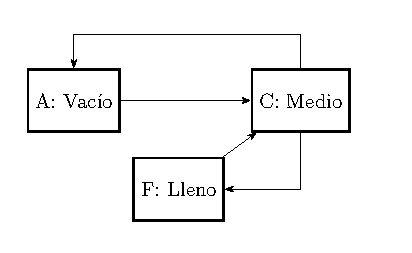
\includegraphics[width=0.7\textwidth]{ImagenesEjercicio1/Bloques-TT.pdf}
	\caption{Finite state machine.}
	\label{fig:fsm}
\end{figure}

Con lo presentado en la Figura (\ref{fig:fsm}), se confecciona una tabla de transiciones.
\begin{table}[H]
\centering
\begin{tabular}{|c|cccc|cc|}
\hline
\textbf{Estado Acutal} & \multicolumn{4}{c|}{\textbf{Estado Futuro}} & \multicolumn{2}{c|}{\textbf{Salida}} \\ \hline
                       & I-S       & I-S       & I-S      & I-S               & Both        & Toggle        \\
                       & 0-0       & 0-1       & 1-0      & 1-1                  &            &           \\ \hline
A                      & x         & x         & B        & x                   & 1          & 0         \\ \cline{1-1}
B                      & A         & x         & x        & C                  & 0          & 1         \\ \cline{1-1}
C                      & x         & x         & B        & x                  & 0        & 0  \\ \hline
\end{tabular}
\caption{Tabla de transiciones del sistema.}
\label{tab:estados}
\end{table}

A partir de la Tabla (\ref{tab:estados}) y la Figura (\ref{fig:fsm}) se puede llegar a la siguiente tabla, donde $y_1$ e $y_2$ representan la salida de los flip-flops, mientras que $Y_1$ e $Y_2$ la entrada de los mismos.
\begin{table}[H]
\centering
\begin{tabular}{|cc|cccc|cc|}
\hline
\textbf{Estado Acutal}  & \textbf{Codificación} & \multicolumn{4}{c}{\textbf{Estado Futuro}}                                                                                                                                                                                                                         & \multicolumn{2}{c|}{\textbf{Salida}} \\ \hline
\multicolumn{1}{|c|}{}  & $y_2 - y_1$           & \begin{tabular}[c]{@{}c@{}}$Y_2 - Y_1$\\ I-S\end{tabular} & \begin{tabular}[c]{@{}c@{}}$Y_2 - Y_1$\\ I-S\end{tabular} & \multicolumn{1}{c|}{\begin{tabular}[c]{@{}c@{}}$Y_2 - Y_1$\\ I-S\end{tabular}} & \begin{tabular}[c]{@{}c@{}}$Y_2 - Y_1$\\ I-S\end{tabular} & Ambos            & Toggle            \\
\multicolumn{1}{|c|}{}  &                       & 0-0                                                       & 0-1                                                       & \multicolumn{1}{c|}{1-0}                                                       & 1-1                                                       &                  &                   \\ \hline
\multicolumn{1}{|c|}{A} & 00                    & x                                                         & x                                                         & 01                                                                             & x                                                         & 1                & 0                 \\ \cline{1-1}
\multicolumn{1}{|c|}{B} & 01                    & 00                                                        & x                                                         & x                                                                              & 11                                                        & 0                & 1                 \\ \cline{1-1}
\multicolumn{1}{|c|}{C} & 10                    & x                                                         & x                                                         & 01                                                                             & x                                                         & 0                & 0                 \\ \cline{1-1}
\multicolumn{1}{|c|}{D} & 11                    & x                                                         & x                                                         & x                                                                              & x                                                         & x                & x                 \\ \hline
\end{tabular}
\end{table}

Se destaca que la variable ``Ambos'' hace referencia a estado en el cual se deben prender ambas bombas, mientras que la variable ``Toggle'' a cuando debe prenderse una sola e intercambiar.

Luego, se prosigue a resolver los mapas de Karnaugh para cada variable:

\begin{figure}[H]
\centering
\begin{subfigure}{.49\textwidth}
\centering
	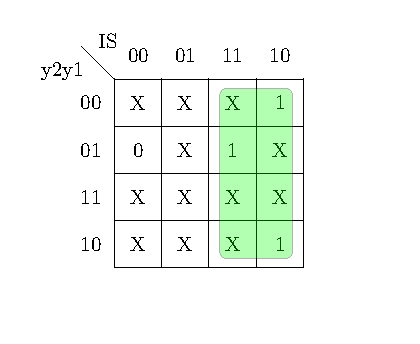
\includegraphics[width=0.7\textwidth]{ImagenesEjercicio1/Mapa1.pdf}
	\caption{Tabla de Karnaugh para $Y_1$.}
	\label{fig:fsm1}
\end{subfigure}
\begin{subfigure}{.49\textwidth}
\centering
	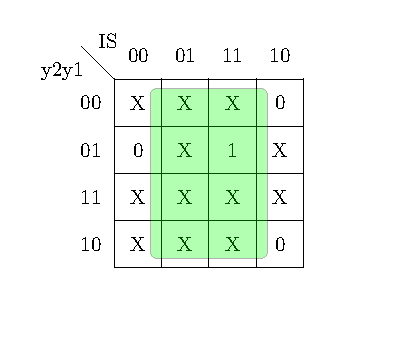
\includegraphics[width=0.7\textwidth]{ImagenesEjercicio1/Mapa2.pdf}
	\caption{Tabla de Karnaugh para $Y_2$.}
	\label{fig:fsm2}
\end{subfigure} \\
\begin{subfigure}{.49\textwidth}
\centering
	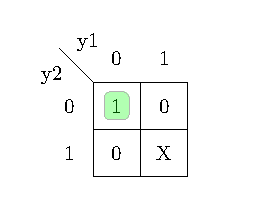
\includegraphics[width=0.5\textwidth]{ImagenesEjercicio1/Mapa3.pdf}
	\caption{Tabla de Karnaugh para ``Ambos''.}
	\label{fig:fsm3}
\end{subfigure}
\begin{subfigure}{.49\textwidth}
\centering
	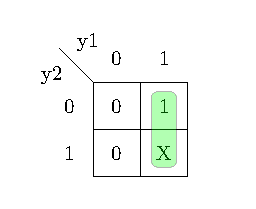
\includegraphics[width=0.5\textwidth]{ImagenesEjercicio1/Mapa4.pdf}
	\caption{Tabla de Karnaugh para ``Toggle''.}
	\label{fig:fsm4}
\end{subfigure}
\caption{Tablas de Karnaugh para cada variable analizada.}
\label{fig:kar}
\end{figure}

A partir de la Figura (\ref{fig:kar}) se derivan las siguientes expresiones:
\begin{equation}
\begin{split}
	Y_1 = & I \\
	Y_2 = & S 
\end{split}
\end{equation}
\begin{equation}
\begin{split}
Ambos = & \ \overline{y_2+y_1} \\
Toggle = & \ y_1
\end{split}
\end{equation}

Luego, se procede a obtener los circuitos para la FSM.
\begin{figure}[H]
\centering
	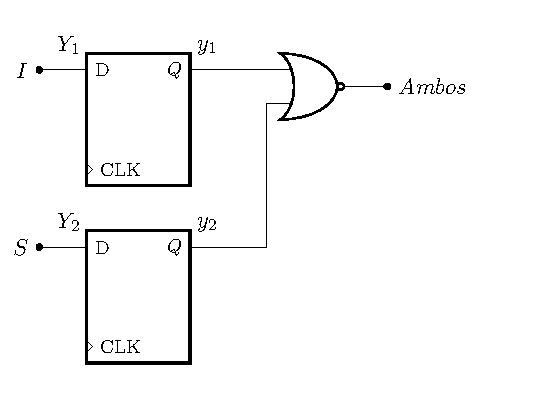
\includegraphics[width=0.6\textwidth, page=1]{ImagenesEjercicio1/Circuitos.pdf}
		\caption{Circuito FSM.}
	\label{fig:fsm1}
\end{figure}

Agregando el siguiente circuito lógico, se implementa la función de Toggle junto a la lógica de salida.
\begin{figure}[H]
	\centering
	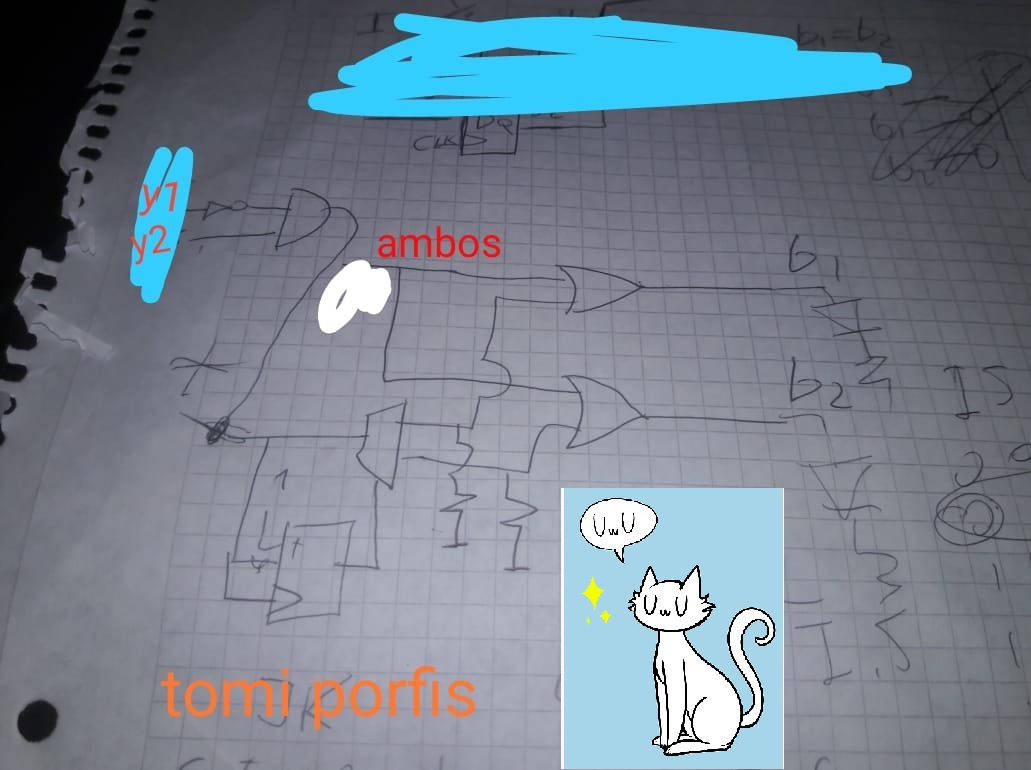
\includegraphics[width=0.7\textwidth]{ImagenesEjercicio1/post_logic.jpeg}
	\caption{Circuito FSM con Toggle.}
	\label{fig:fsm2}
\end{figure}
A partir de estos circuitos se realizó el PCB del mismo:
 \begin{figure}[H]
	\centering
	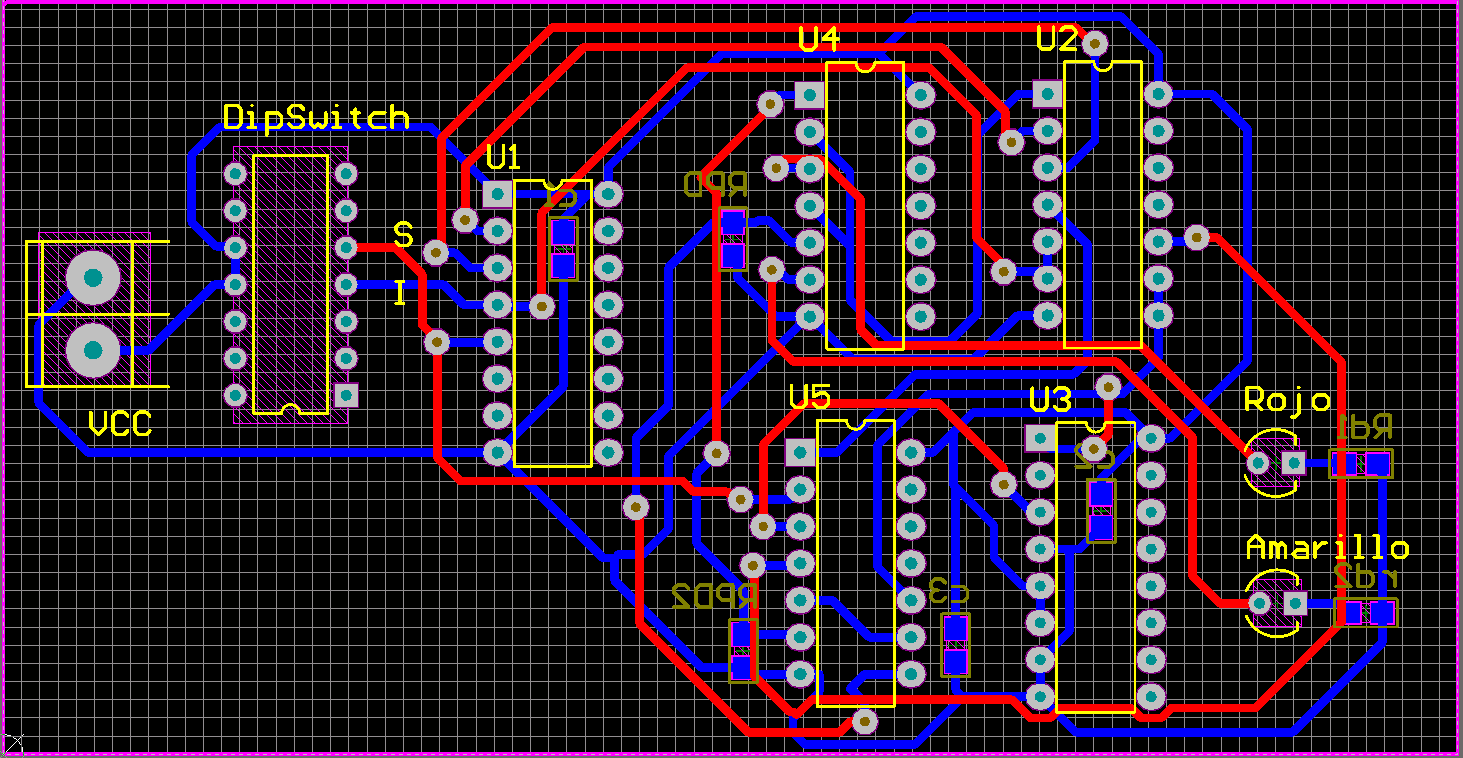
\includegraphics[width=0.7\textwidth]{ImagenesEjercicio1/PCB.PNG}
	\caption{PCB.}
	\label{fig:fsm}
\end{figure}
Dicha placa se llevo a cabo con resultados positivos.
 \begin{figure}[H]
	\centering
	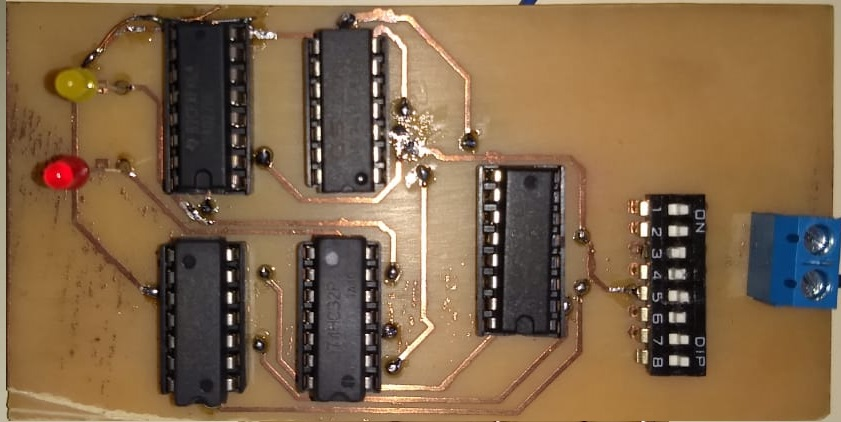
\includegraphics[width=0.8\textwidth]{ImagenesEjercicio1/pcbReal.jpeg}
	\caption{PCB implementado.}
	\label{fig:fsm}
\end{figure}
Luego se proecidió a medir los niveles de tensión para las transiciones posibles:
 \begin{figure}[H]
	\centering
	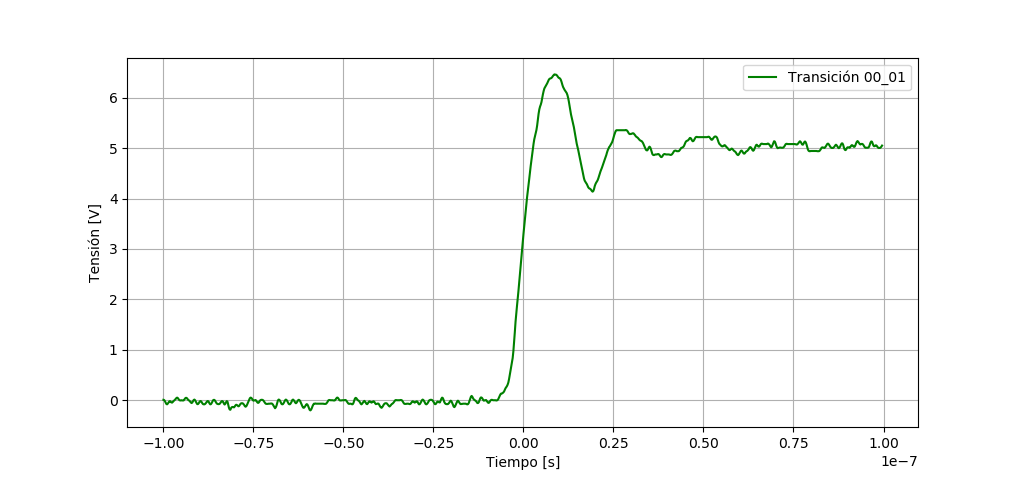
\includegraphics[width=0.8\textwidth]{ImagenesEjercicio1/00-01.PNG}
	\caption{Transición 00-01.}
	\label{fig:0001}
\end{figure}
 \begin{figure}[H]
	\centering
	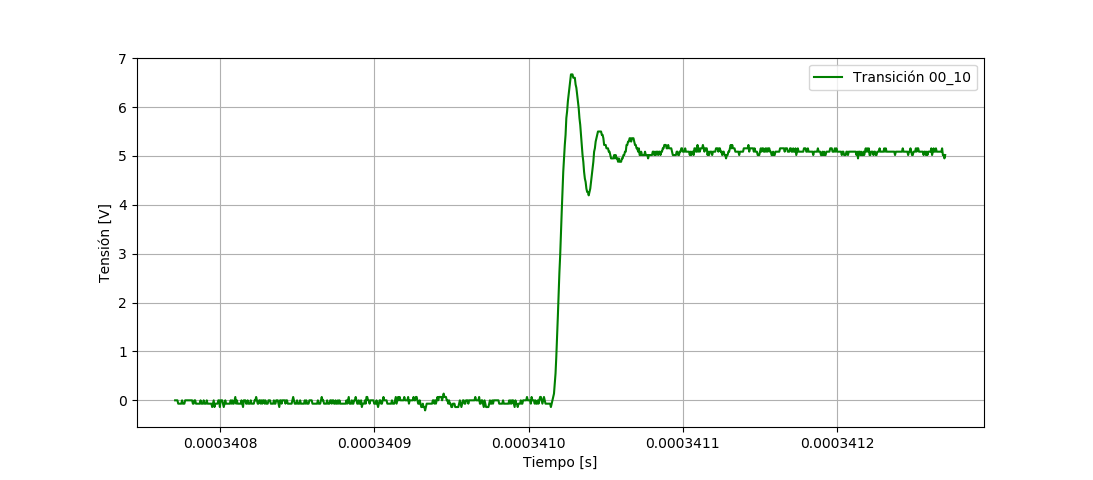
\includegraphics[width=0.8\textwidth]{ImagenesEjercicio1/00-10.PNG}
	\caption{Transición 00-10.}
	\label{fig:0010}
\end{figure}
 \begin{figure}[H]
	\centering
	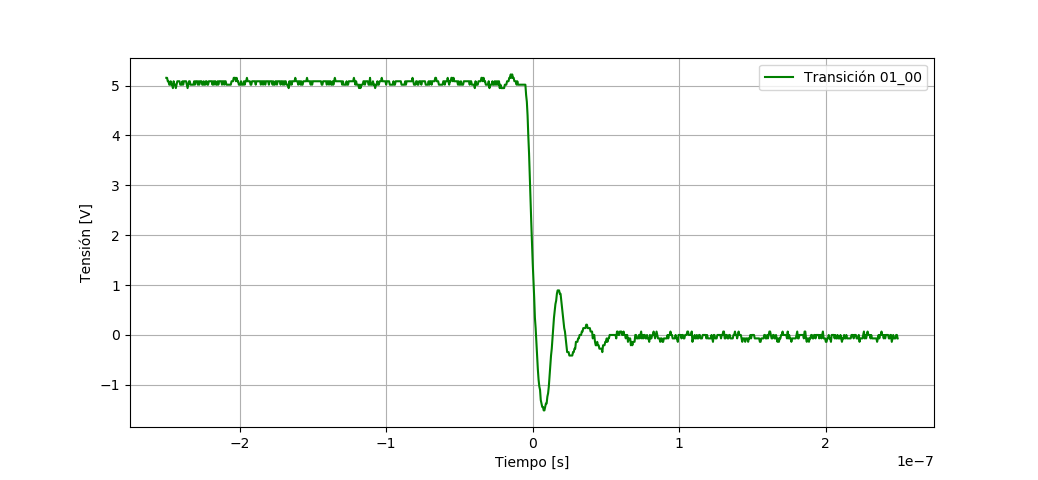
\includegraphics[width=0.8\textwidth]{ImagenesEjercicio1/01-00.PNG}
	\caption{Transición 01-00.}
	\label{fig:0100}
\end{figure}
 \begin{figure}[H]
	\centering
	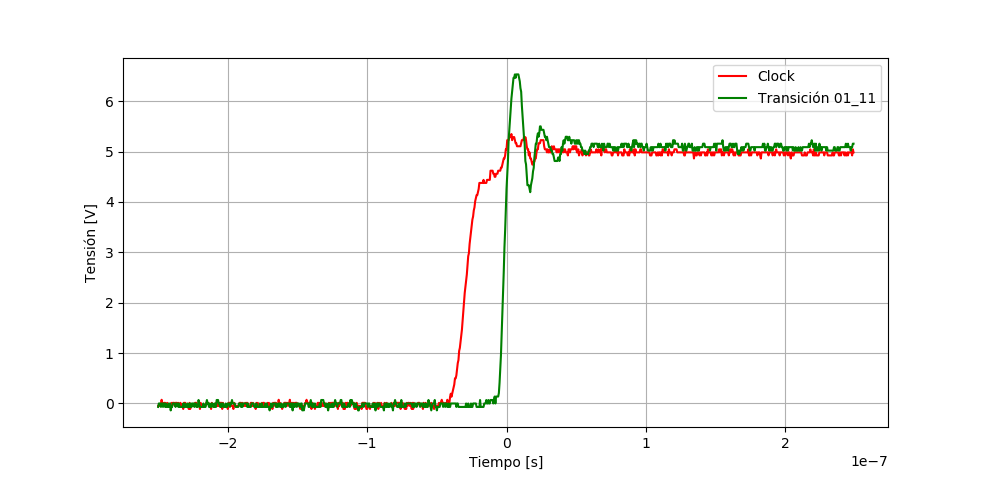
\includegraphics[width=0.8\textwidth]{ImagenesEjercicio1/01-11.PNG}
	\caption{Transición 01-11.}
	\label{fig:0111}
\end{figure}
 \begin{figure}[H]
	\centering
	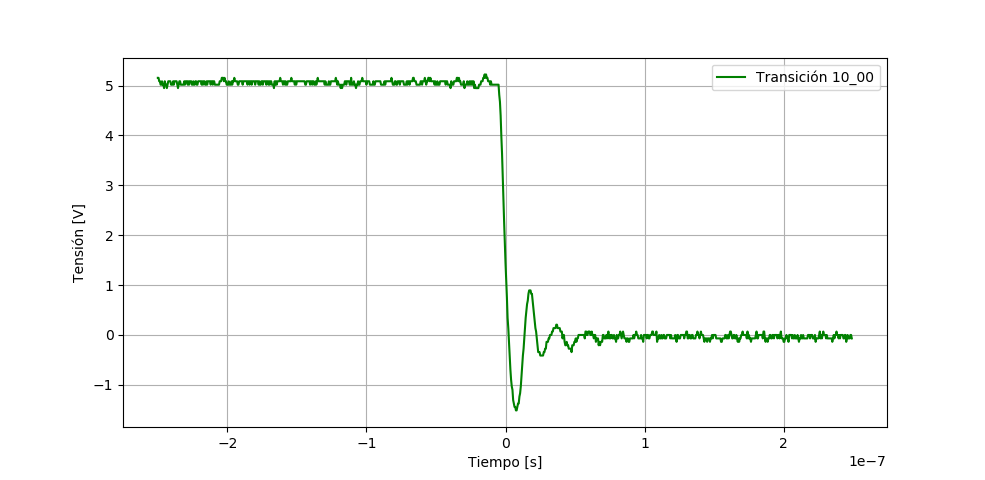
\includegraphics[width=0.8\textwidth]{ImagenesEjercicio1/10-00.PNG}
	\caption{Transición 10-00.}
	\label{fig:1000}
\end{figure}
 \begin{figure}[H]
	\centering
	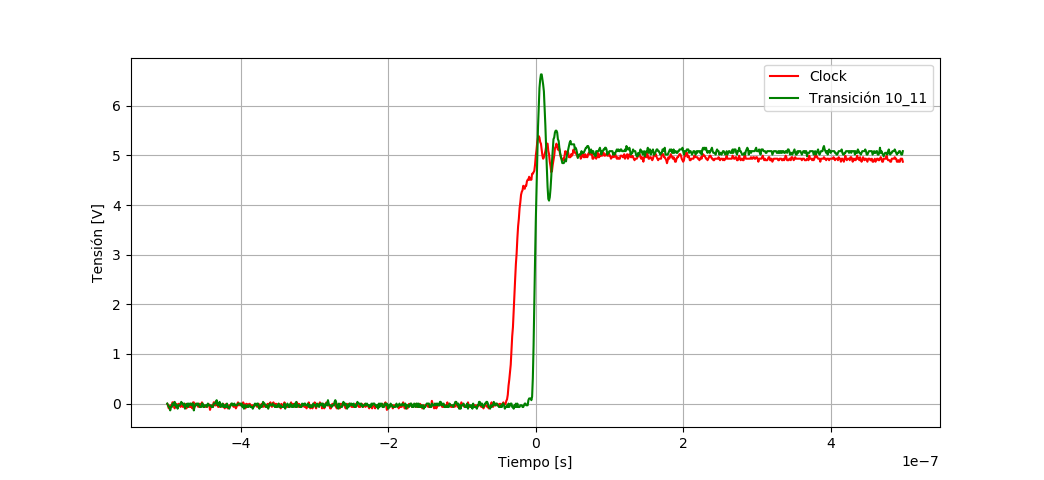
\includegraphics[width=0.8\textwidth]{ImagenesEjercicio1/10-11.PNG}
	\caption{Transición 10-11.}
	\label{fig:1011}
\end{figure}
 \begin{figure}[H]
	\centering
	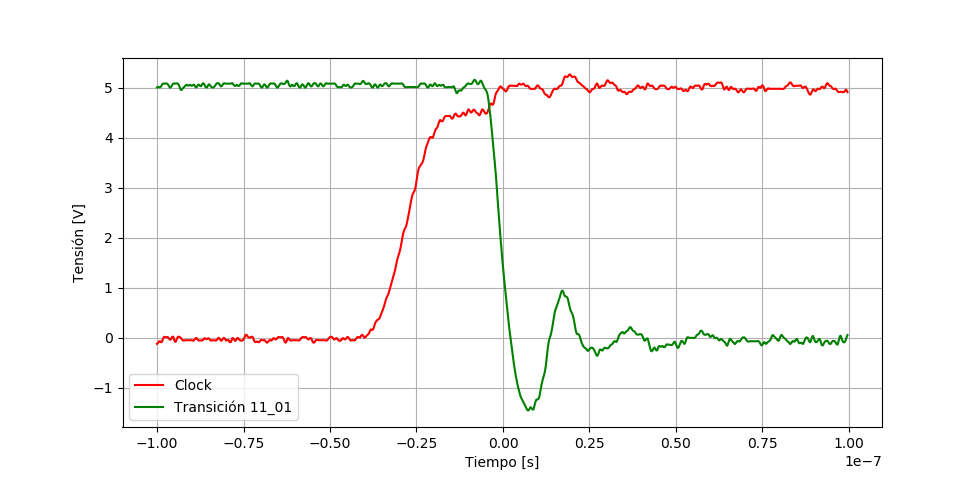
\includegraphics[width=0.8\textwidth]{ImagenesEjercicio1/11-01.PNG}
	\caption{Transición 11-01.}
	\label{fig:1101}
\end{figure}
 \begin{figure}[H]
	\centering
	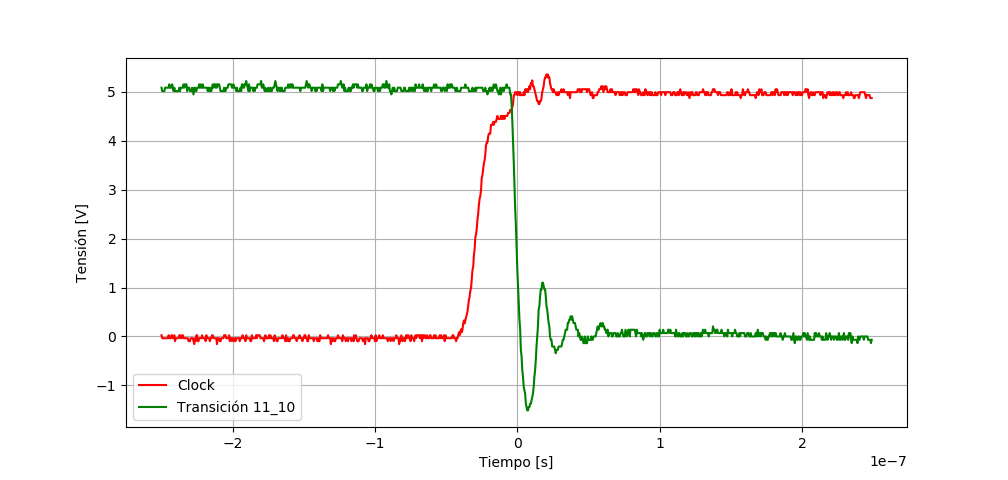
\includegraphics[width=0.8\textwidth]{ImagenesEjercicio1/11-10.PNG}
	\caption{Transición 11-10.}
	\label{fig:1110}
\end{figure}
\end{document}
		
\section{Ejercicio 2}
	\label{Ejercicio-2}
%	\documentclass[a4paper]{article}
\usepackage[utf8]{inputenc}
\usepackage[spanish, es-tabla, es-noshorthands]{babel}
\usepackage[table,xcdraw]{xcolor}
\usepackage[a4paper, footnotesep = 1cm, width=18cm, left=2cm, top=2.5cm, height=25cm, textwidth=18cm, textheight=25cm]{geometry}
%\geometry{showframe}

\usepackage{tikz}
\usepackage{amsmath}
\usepackage{amsfonts}
\usepackage{amssymb}
\usepackage{float}
\usepackage{graphicx}
\usepackage{caption}
\usepackage{subcaption}
\usepackage{multicol}
\usepackage{multirow}
\setlength{\doublerulesep}{\arrayrulewidth}
\usepackage{booktabs}

\usepackage{hyperref}
\hypersetup{
    colorlinks=true,
    linkcolor=blue,
    filecolor=magenta,      
    urlcolor=blue,
    citecolor=blue,    
}
\newcommand\underrel[2]{\mathrel{\mathop{#2}\limits_{#1}}}
\newcommand{\quotes}[1]{``#1''}
\usepackage{array}
\newcolumntype{C}[1]{>{\centering\let\newline\\\arraybackslash\hspace{0pt}}m{#1}}
\usepackage[american]{circuitikz}
\usetikzlibrary{calc}
\usepackage{fancyhdr}
\usepackage{units} 

\graphicspath{{../Ejercicio-1/}{../Ejercicio-2/}{../Ejercicio-3/}}

\pagestyle{fancy}
\fancyhf{}
\lhead{22.13 Electrónica III}
\rhead{Mechoulam, Lambertucci, Martorell, Londero}
\rfoot{\center \thepage}
\usepackage{multirow}
\begin{document}

\section{Ejercicio 2}
\subsection{Introdución}
En esta sección se procederá a realizar una máquina de estados capaz de detectar la secuencia de bits 1-1-0-1.

\subsection{Implementación} 
Para poder realizar esta detector de secuencias se consideró que el último bit de la secuencia puede ser el primero de una nueva, por ejemplo, si viene una cadena de bits de la siguiente forma 1-1-0-1-1-0-1 la máquina de estados detectará dos secuencias correctas de bits. A su vez se consideró que si un caracter es incorrecto la máquina de estado vuelve a su estado base inicial y se vuelve a comenzar. Se realizo el siguiente diagrama de estados utilizando una máquina de Mealy:
\begin{figure}[H]
\centering

\includegraphics{ImagenesEjercicio2/pend.jpg}
\caption{Diagrama de la máquina de Mealy utilizada para detectar la secuencia de bits}
\end{figure}


Otorgandole a los estados la siguiente numeración: $A=00$, $B=01$, $C=10$, $D=11$, se obtiene la siguiente tabla:

\begin{table}[H]
\centering
\begin{tabular}{ccccc}
\multirow{2}{*}{Estado actual} & \multicolumn{2}{c}{Próximo estado} & \multicolumn{2}{c}{Salida} \\
 & w=0 & w=1 & w=0 & w=1 \\
$y_2y_1$ & $Y_2Y_1$ & $Y_2Y_1$ & $Z$ & $Z$ \\
A & A(00) & B(01) & 0 & 0 \\
B & A(00) & C(10) & 0 & 0 \\
C & D(11) & A(00) & 0 & 0 \\
D & A(00) & B(01) & 0 & 1
\end{tabular}
\end{table}

A partir de esta tabla se realizaron los respectivos mapas de karnaugh para las salidas $Y_1$, $Y_2$, se pudo observar que tanto para maxtérminos como para mintérminos el número de operaciones lógicas a realizar eran las mismas, por lo tanto se optó por utilizar los mintérminos y se obtuvo los siguientes mapas:

\begin{figure}[H]
\centering
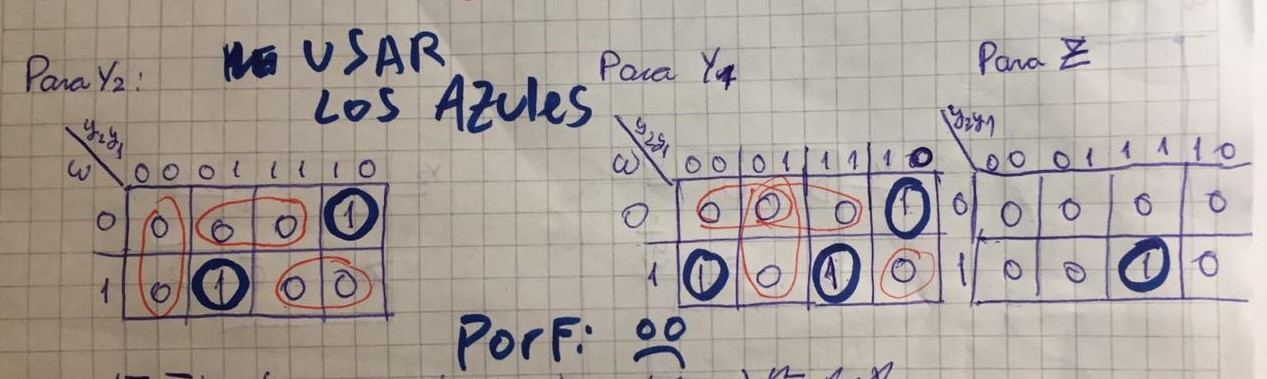
\includegraphics{ImagenesEjercicio2/mapitas.jpg}
\caption{Mapas de karnaugh primero del primer Flip-Flop, luego del segundo y por último la salida deseada}
\end{figure}
Con los que se obtienen las siguientes funciones:
$Y_1=(w\bar{y_2}\bar{y_1})+(wy_1y_2)+(\bar{w}y_2\bar{y_1})$
$Y_2=(w\bar{y_2}y_1)+(\bar{w}y_2\bar{y_1})$
$Z=wy_2y_1$
Utilizando 2 flip-flops tipo D para representar las 4 combinaciones posibles para obtener todos los posibles estados, considerando que los proximos estados se pueden representar como la entrada de dichos flip-flops y la salida de estos como el estado actual, se presenta el siguiente circuito:
\begin{figure}[H]
\centering
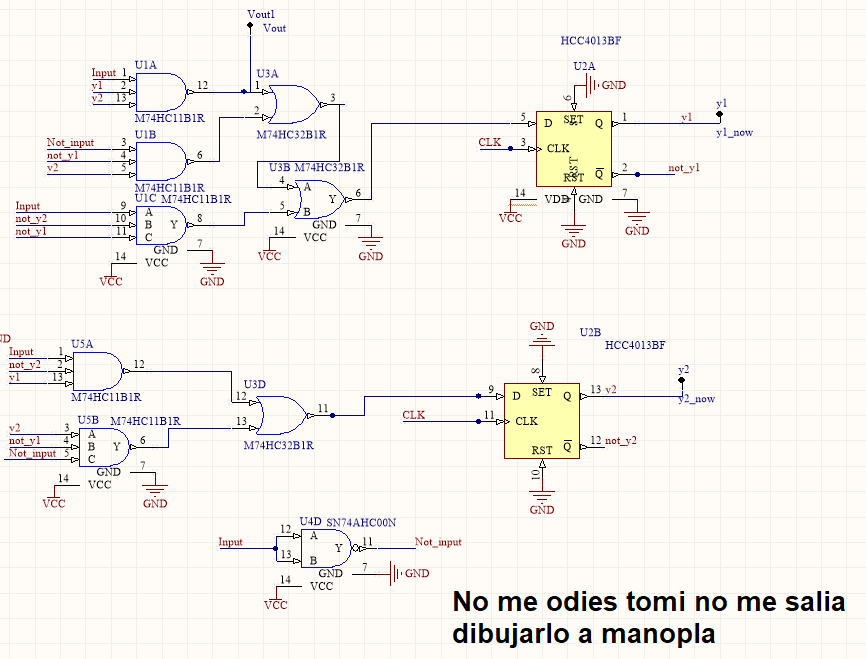
\includegraphics{ImagenesEjercicio2/circuito.jpg}
\caption{Circuito a implimitar que cumple con la maquina de estados deseada}
\end{figure}
\end{document}

Consecuentemente se procedio a realizar la simulación en verilog de dicho circuito con la que se obtuvo los siguientes resultados:

\begin{figure}[H]
\centering
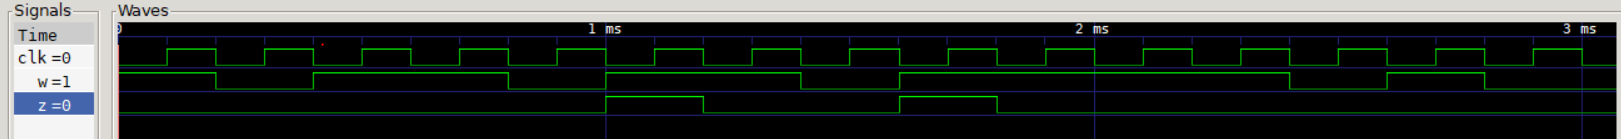
\includegraphics{ImagenesEjercicio2/simulacion.png}
\caption{Simulaciones en GTKwave, donde w simboliza la entrada, z la salida y clk el clock del circuito}
\end{figure}
\end{document}

Como era de esperarse dicho circuito emula satisfactoriamente la máquina de estados planteada, por lo que se puede detectar correctamente la secuencia de bits deseados cuando esta se presenta. Ulteriormente de las simulaciones se procedio a diseñar dicho circuito en PCB con el cual se obtuvieron los mismos resultados por lo que se corroboró el correcto funcionamiento de la máquina de estados implementada, como se puede presenciar en las siguientes figuras.

\begin{figure}[H]
\centering
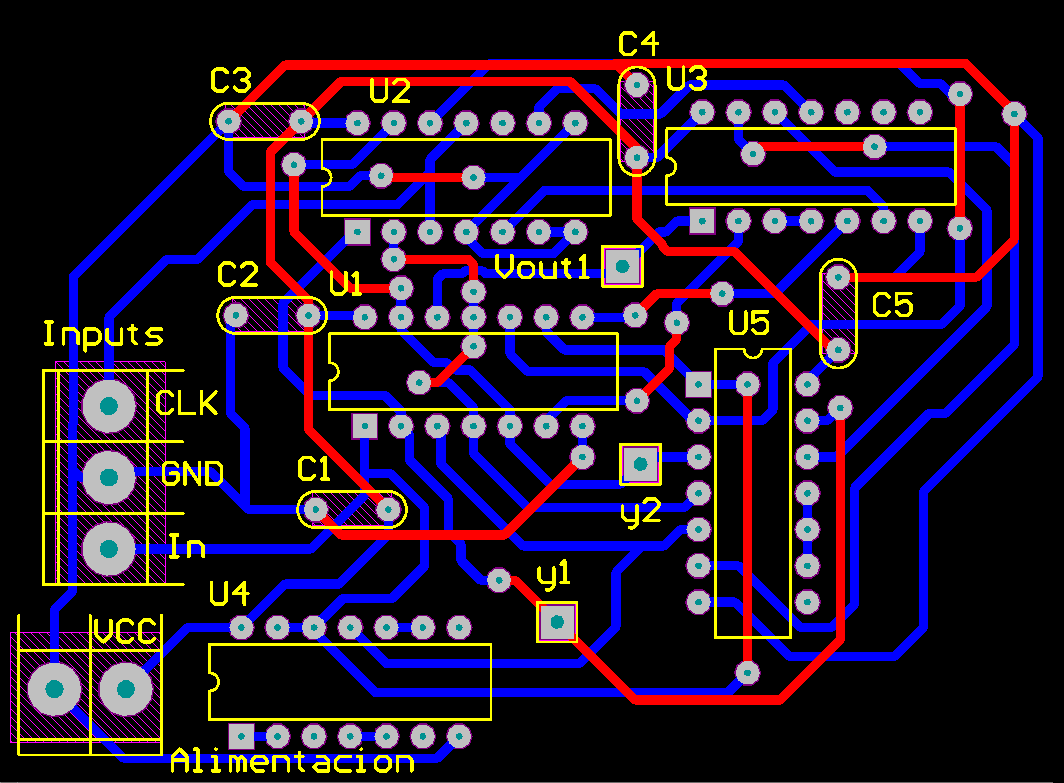
\includegraphics{ImagenesEjercicio2/pcb.png}
\caption{Implementación en PCB del circuito implementado }
\end{figure}
\end{document}

\begin{figure}[H]
\centering

\includegraphics{ImagenesEjercicio2/pend.jpg}
\caption{Detección de la secuencia deseada vista en el osciloscopio }
\end{figure}
\end{document}


	
\section{Ejercicio 3}
	\label{Ejercicio-3}
%	\documentclass[a4paper]{article}
\usepackage[utf8]{inputenc}
\usepackage[spanish, es-tabla, es-noshorthands]{babel}
\usepackage[table,xcdraw]{xcolor}
\usepackage[a4paper, footnotesep = 1cm, width=18cm, left=2cm, top=2.5cm, height=25cm, textwidth=18cm, textheight=25cm]{geometry}
%\geometry{showframe}

\usepackage{tikz}
\usepackage{amsmath}
\usepackage{amsfonts}
\usepackage{amssymb}
\usepackage{float}
\usepackage{graphicx}
\usepackage{caption}
\usepackage{subcaption}
\usepackage{multicol}
\usepackage{multirow}
\setlength{\doublerulesep}{\arrayrulewidth}
\usepackage{booktabs}

\usepackage{hyperref}
\hypersetup{
    colorlinks=true,
    linkcolor=blue,
    filecolor=magenta,      
    urlcolor=blue,
    citecolor=blue,    
}
\newcommand\underrel[2]{\mathrel{\mathop{#2}\limits_{#1}}}
\newcommand{\quotes}[1]{``#1''}
\usepackage{array}
\newcolumntype{C}[1]{>{\centering\let\newline\\\arraybackslash\hspace{0pt}}m{#1}}
\usepackage[american]{circuitikz}
\usetikzlibrary{calc}
\usepackage{fancyhdr}
\usepackage{units} 

\graphicspath{{../Ejercicio-1/}{../Ejercicio-2/}{../Ejercicio-3/}}

\pagestyle{fancy}
\fancyhf{}
\lhead{22.13 Electrónica III}
\rhead{Mechoulam, Lambertucci, Martorell, Londero}
\rfoot{\center \thepage}
\usepackage{tikz}
\usetikzlibrary{matrix,calc}

%isolated term
%#1 - Optional. Space between node and grouping line. Default=0
%#2 - node
%#3 - filling color
\newcommand{\implicantsol}[3][0]{
    \draw[rounded corners=3pt, fill=#3, opacity=0.3] ($(#2.north west)+(135:#1)$) rectangle ($(#2.south east)+(-45:#1)$);
    }


%internal group
%#1 - Optional. Space between node and grouping line. Default=0
%#2 - top left node
%#3 - bottom right node
%#4 - filling color
\newcommand{\implicant}[4][0]{
    \draw[rounded corners=3pt, fill=#4, opacity=0.3] ($(#2.north west)+(135:#1)$) rectangle ($(#3.south east)+(-45:#1)$);
    }

%group lateral borders
%#1 - Optional. Space between node and grouping line. Default=0
%#2 - top left node
%#3 - bottom right node
%#4 - filling color
\newcommand{\implicantcostats}[4][0]{
    \draw[rounded corners=3pt, fill=#4, opacity=0.3] ($(rf.east |- #2.north)+(90:#1)$)-| ($(#2.east)+(0:#1)$) |- ($(rf.east |- #3.south)+(-90:#1)$);
    \draw[rounded corners=3pt, fill=#4, opacity=0.3] ($(cf.west |- #2.north)+(90:#1)$) -| ($(#3.west)+(180:#1)$) |- ($(cf.west |- #3.south)+(-90:#1)$);
}

%group top-bottom borders
%#1 - Optional. Space between node and grouping line. Default=0
%#2 - top left node
%#3 - bottom right node
%#4 - filling color
\newcommand{\implicantdaltbaix}[4][0]{
    \draw[rounded corners=3pt, fill=#4, opacity=0.3] ($(cf.south -| #2.west)+(180:#1)$) |- ($(#2.south)+(-90:#1)$) -| ($(cf.south -| #3.east)+(0:#1)$);
    \draw[rounded corners=3pt, fill=#4, opacity=0.3] ($(rf.north -| #2.west)+(180:#1)$) |- ($(#3.north)+(90:#1)$) -| ($(rf.north -| #3.east)+(0:#1)$);
}

%group corners
%#1 - Optional. Space between node and grouping line. Default=0
%#2 - filling color
\newcommand{\implicantcantons}[2][0]{
    \draw[rounded corners=3pt, opacity=.3] ($(rf.east |- 0.south)+(-90:#1)$) -| ($(0.east |- cf.south)+(0:#1)$);
    \draw[rounded corners=3pt, opacity=.3] ($(rf.east |- 8.north)+(90:#1)$) -| ($(8.east |- rf.north)+(0:#1)$);
    \draw[rounded corners=3pt, opacity=.3] ($(cf.west |- 2.south)+(-90:#1)$) -| ($(2.west |- cf.south)+(180:#1)$);
    \draw[rounded corners=3pt, opacity=.3] ($(cf.west |- 10.north)+(90:#1)$) -| ($(10.west |- rf.north)+(180:#1)$);
    \fill[rounded corners=3pt, fill=#2, opacity=.3] ($(rf.east |- 0.south)+(-90:#1)$) -|  ($(0.east |- cf.south)+(0:#1)$) [sharp corners] ($(rf.east |- 0.south)+(-90:#1)$) |-  ($(0.east |- cf.south)+(0:#1)$) ;
    \fill[rounded corners=3pt, fill=#2, opacity=.3] ($(rf.east |- 8.north)+(90:#1)$) -| ($(8.east |- rf.north)+(0:#1)$) [sharp corners] ($(rf.east |- 8.north)+(90:#1)$) |- ($(8.east |- rf.north)+(0:#1)$) ;
    \fill[rounded corners=3pt, fill=#2, opacity=.3] ($(cf.west |- 2.south)+(-90:#1)$) -| ($(2.west |- cf.south)+(180:#1)$) [sharp corners]($(cf.west |- 2.south)+(-90:#1)$) |- ($(2.west |- cf.south)+(180:#1)$) ;
    \fill[rounded corners=3pt, fill=#2, opacity=.3] ($(cf.west |- 10.north)+(90:#1)$) -| ($(10.west |- rf.north)+(180:#1)$) [sharp corners] ($(cf.west |- 10.north)+(90:#1)$) |- ($(10.west |- rf.north)+(180:#1)$) ;
}

%Empty Karnaugh map 4x4
\newenvironment{Karnaugh}%
{
\begin{tikzpicture}[baseline=(current bounding box.north),scale=0.8]
\draw (0,0) grid (4,4);
\draw (0,4) -- node [pos=0.7,above right,anchor=south west] {ba} node [pos=0.7,below left,anchor=north east] {dc} ++(135:1);
%
\matrix (mapa) [matrix of nodes,
        column sep={0.8cm,between origins},
        row sep={0.8cm,between origins},
        every node/.style={minimum size=0.3mm},
        anchor=8.center,
        ampersand replacement=\&] at (0.5,0.5)
{
                       \& |(c00)| 00         \& |(c01)| 01         \& |(c11)| 11         \& |(c10)| 10         \& |(cf)| \phantom{00} \\
|(r00)| 00             \& |(0)|  \phantom{0} \& |(1)|  \phantom{0} \& |(3)|  \phantom{0} \& |(2)|  \phantom{0} \&                     \\
|(r01)| 01             \& |(4)|  \phantom{0} \& |(5)|  \phantom{0} \& |(7)|  \phantom{0} \& |(6)|  \phantom{0} \&                     \\
|(r11)| 11             \& |(12)| \phantom{0} \& |(13)| \phantom{0} \& |(15)| \phantom{0} \& |(14)| \phantom{0} \&                     \\
|(r10)| 10             \& |(8)|  \phantom{0} \& |(9)|  \phantom{0} \& |(11)| \phantom{0} \& |(10)| \phantom{0} \&                     \\
|(rf) | \phantom{00}   \&                    \&                    \&                    \&                    \&                     \\
};
}%
{
\end{tikzpicture}
}

%Empty Karnaugh map 2x4
\newenvironment{Karnaughvuit}%
{
\begin{tikzpicture}[baseline=(current bounding box.north),scale=0.8]
\draw (0,0) grid (4,2);
\draw (0,2) -- node [pos=0.7,above right,anchor=south west] {bc} node [pos=0.7,below left,anchor=north east] {a} ++(135:1);
%
\matrix (mapa) [matrix of nodes,
        column sep={0.8cm,between origins},
        row sep={0.8cm,between origins},
        every node/.style={minimum size=0.3mm},
        anchor=4.center,
        ampersand replacement=\&] at (0.5,0.5)
{
                      \& |(c00)| 00         \& |(c01)| 01         \& |(c11)| 11         \& |(c10)| 10         \& |(cf)| \phantom{00} \\
|(r00)| 0             \& |(0)|  \phantom{0} \& |(1)|  \phantom{0} \& |(3)|  \phantom{0} \& |(2)|  \phantom{0} \&                     \\
|(r01)| 1             \& |(4)|  \phantom{0} \& |(5)|  \phantom{0} \& |(7)|  \phantom{0} \& |(6)|  \phantom{0} \&                     \\
|(rf) | \phantom{00}  \&                    \&                    \&                    \&                    \&                     \\
};
}%
{
\end{tikzpicture}
}

%Empty Karnaugh map 2x2
\newenvironment{Karnaughquatre}%
{
\begin{tikzpicture}[baseline=(current bounding box.north),scale=0.8]
\draw (0,0) grid (2,2);
\draw (0,2) -- node [pos=0.7,above right,anchor=south west] {b} node [pos=0.7,below left,anchor=north east] {a} ++(135:1);
%
\matrix (mapa) [matrix of nodes,
        column sep={0.8cm,between origins},
        row sep={0.8cm,between origins},
        every node/.style={minimum size=0.3mm},
        anchor=2.center,
        ampersand replacement=\&] at (0.5,0.5)
{
          \& |(c00)| 0          \& |(c01)| 1  \\
|(r00)| 0 \& |(0)|  \phantom{0} \& |(1)|  \phantom{0} \\
|(r01)| 1 \& |(2)|  \phantom{0} \& |(3)|  \phantom{0} \\
};
}%
{
\end{tikzpicture}
}

%Defines 8 or 16 values (0,1,X)
\newcommand{\contingut}[1]{%
\foreach \x [count=\xi from 0]  in {#1}
     \path (\xi) node {\x};
}

%Places 1 in listed positions
\newcommand{\minterms}[1]{%
    \foreach \x in {#1}
        \path (\x) node {1};
}

%Places 0 in listed positions
\newcommand{\maxterms}[1]{%
    \foreach \x in {#1}
        \path (\x) node {0};
}

%Places X in listed positions
\newcommand{\indeterminats}[1]{%
    \foreach \x in {#1}
        \path (\x) node {X};
}

% \begin{document}
%     \begin{Karnaugh}
%         \contingut{0,0,0,0,0,0,0,0,0,0,0,0,0,0,0,0}
%        \implicant{0}{2}{red}
%        \implicant{5}{15}{purple}
%        \implicantdaltbaix[3pt]{3}{10}{blue}
%     \implicantcantons[2pt]{orange}
%        \implicantcostats{4}{14}{green}
%     \end{Karnaugh}
%     %
%     \begin{Karnaughvuit}
%        \minterms{3,4}
%         \maxterms{0,1,6,7}
%        \indeterminats{2,5}
%        \implicant{3}{2}{green}
%        \implicant{4}{5}{}
%     \end{Karnaughvuit}
%     %
%     \begin{Karnaughquatre}
%         \minterms{1,2}
%        \maxterms{0,3}
%        \implicantsol{1}{green}
%        \implicantsol{2}{red}
%     \end{Karnaughquatre}

% \end{document}
\begin{document}

\subsection{Introducción}

Se quiso implementar la siguiente máquina de estados finitos:

\begin{figure}[H]
\centering
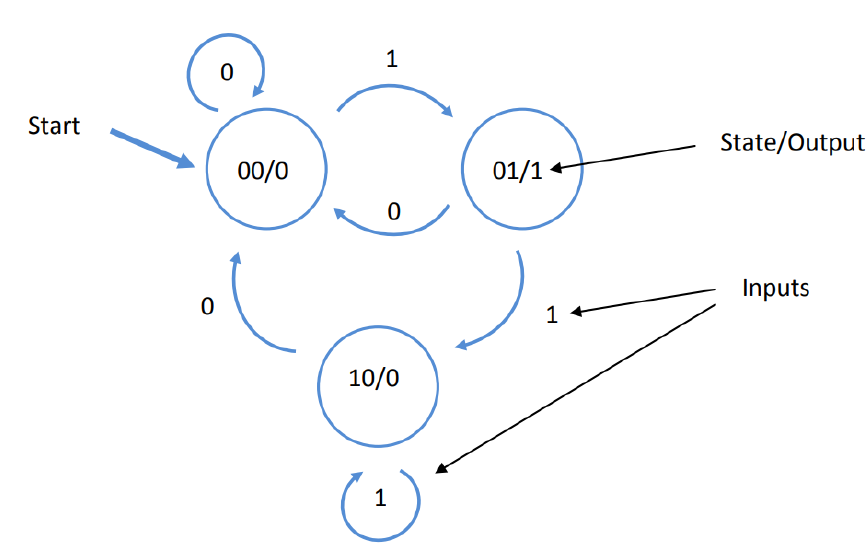
\includegraphics[width=0.6\textwidth]{ImagenesEjercicio3/fsm.png}
\caption{Máquina de estados finitos a implementar.}
\label{fig:fsm}
\end{figure} 

Para esto, se conformó la tabla de estados considerando al estado $00$ como el inicial, resultando:

\begin{table}[H]
\centering
\begin{tabular}{|c|l|c|l|c|l|c|}
\hline
\multicolumn{2}{|c|}{\multirow{2}{*}{$Present State$}} & \multicolumn{4}{c|}{$Next State$} & \multirow{3}{*}{$Output (z)$} \\ \cline{3-6}
\multicolumn{2}{|c|}{} & \multicolumn{2}{c|}{$w=0$} & \multicolumn{2}{c|}{$w=1$} &  \\
\multicolumn{2}{|c|}{$y_2 y_1$} & \multicolumn{2}{c|}{$Y_2Y_1$} & \multicolumn{2}{c|}{$Y_2Y_1$} &  \\ \hline
\multicolumn{2}{|c|}{00} & \multicolumn{2}{c|}{00} & \multicolumn{2}{c|}{01} & 0 \\ \hline
\multicolumn{2}{|c|}{01} & \multicolumn{2}{c|}{00} & \multicolumn{2}{c|}{10} & 1 \\ \hline
\multicolumn{2}{|c|}{10} & \multicolumn{2}{c|}{00} & \multicolumn{2}{c|}{10} & 0 \\ \hline
\multicolumn{2}{|c|}{11} & \multicolumn{2}{c|}{xx} & \multicolumn{2}{c|}{xx} & x \\ \hline
\end{tabular}
\caption{Tabla de estados para la máquina de estados finita a implementar.}
\label{fig:tablaestados}
\end{table}

Como fue necesario implementar tres estados se requirió utilizar dos flip-flops. Luego, se hallaron las fórmulas lógicas para los estados siguientes utilizando mapas de karnaugh.

\begin{figure}[H]
\begin{subfigure}{0.49\textwidth}
\begin{centering}
    \begin{Karnaughvuit}
        \minterms{5, 6}
        \maxterms{0,1,2,4}
        \indeterminats{7, 3}
        
        \implicant{5}{7}{orange}
        \implicant{7}{6}{blue}
        
    \end{Karnaughvuit}
\par\end{centering}
\begin{equation*}
Y_2 = wy_1+wy_2
\end{equation*}
\begin{table}[H]
\caption{Solución para $Y_2.$}
\label{mapa:Y2}
\end{table}
\end{subfigure}
\begin{subfigure}{0.49\textwidth}
\begin{centering}
    \begin{Karnaughvuit}
        \minterms{4}
        \maxterms{0,1,2,5,6}
        \indeterminats{7,3}
        
        \implicantsol{4}{green}
        
    \end{Karnaughvuit}
\par\end{centering}
\begin{equation*}
Y_1 = w(\overline{y_2}\cdot \overline{y_1})
\end{equation*}
\begin{table}[H]
\caption{Solución para $Y_1.$}
\label{mapa:Y1}
\end{table}
\end{subfigure}
\caption{Mapas de Karnaugh para los próximos estados de la maquina de estados finitos.}
\end{figure}

Utilizando el teorema de DeMorgan y simplificando se obtienen dos posibles implementaciones análogas:
\begin{figure}[H]
\begin{subfigure}{0.49\textwidth}
\vspace*{-0.17cm}
\begin{equation*}
\left.\left\{
\begin{aligned}
		& Y_1 = w(\overline{y_2}\cdot \overline{y_1})	 \\		
		& Y_2 = w\overline{(\overline{y_2}\cdot \overline{y_1})}\\		
\end{aligned}
\right.\right\}
\end{equation*}
\caption{Implementación con NAND.}
\end{subfigure}
\begin{subfigure}{0.49\textwidth}
\begin{equation*}
\left.\left\{
\begin{aligned}
		& Y_1 = w(\overline{y_2+y_1}) \\		
		& Y_2 = w(y_2+y_1)\\		
\end{aligned}
\right.\right\}
\end{equation*}
\caption{Implementación con AND y NOR.}
\end{subfigure}
\end{figure}

Si este circuito fuese trabajado directamente sobre el silicio, se elegiría la implementación con NAND ya que sería la más simple de realizar. Sin embargo, como se contruirá un PCB, se decidió utilizar la implementación con AND y NOR ya que se deberían de utilizar solamente dos integrados para el circuito lógico de entrada y salida, a diferencia de la implementación con NAND, que requeriría de tres integrados (utilizando un total de nueve NAND's). Finalmente, a partir de las ecuaciones obtenidas se esquematizó la implementación teórica.

\begin{figure}[H]
	\hspace*{1cm}
	\centering
	\begin{circuitikz}
		\draw
			
			(0,0)
			node[fourport](FF1){}
				(FF1.1) ++ (0.12,0) node[]{\scalebox{1.2}{\rotatebox{-90}{$\triangle$}}}
				 ++ (-0.12,0) node[](FF1_CLK){}
				(FF1.2) ++ (-0.25, 0) node[](){$\overline{y_1}$}
				node[](FF1_2){}
				(FF1.3) ++ (-0.25, 0) node[](){$y_1$}
				node[](FF1_3){}
				(FF1.4) ++ (0.25, 0) node[](){$Y_1$}
				node[](FF1_4){}
				(FF1_CLK) to[short] ++ (-0.5, 0)
					node[](FF1_CLK){}
				(FF1.3) to[short] ++ (0.5, 0)
					node[](FF1_y){}
				(FF1.4) to[short] ++ (-0.5, 0)
					node[](FF1_Y){}
					
				
			(0,-3)
			node[fourport](FF2){}
				(FF2.1) ++ (0.12,0) node[]{\scalebox{1.2}{\rotatebox{-90}{$\triangle$}}}
				 ++ (-0.12,0) node[](FF2_CLK){}
				(FF2.2) ++ (-0.25, 0) node[](){$\overline{y_2}$}
				node[](FF2_-y){}
				(FF2.3) ++ (-0.25, 0) node[](){$y_2$}
				node[](FF2_y){}
				(FF2.4) ++ (0.25, 0) node[](){$Y_2$}
				node[](FF2_Y){}
				(FF2_CLK) to[short] ++ (-0.5, 0)
					node[](FF2_CLK){}
				(FF2.2) to[short] ++ (0.5, 0)
					node[](FF2_-y){}
				(FF2.3) to[short] ++ (1, 0)
					node[](FF2_y){}
				(FF2.4) to[short] ++ (-0.5, 0)
					node[](FF2_Y){}		
					
					
			(-4, -4)node[ocirc, label=west:$CLK$](CLK){}
				(CLK) to[short] ++ (2.5,0) |-(FF2_CLK.center)
				(CLK) to[open, -*]++(2.5, 0.55) |-(FF1_CLK.center)
				
			(FF1_Y) ++ (-0.5, 0) node[and port, xscale=0.7, yscale=0.7](and1){}
			(and1.in 1) ++ (-0.5, 0) node[nor port, xscale=0.7, yscale=0.7](nor1){}
			
			(FF2_Y) ++ (-0.5, 0) node[and port, xscale=0.7, yscale=0.7](and2){}
			(and2.in 2) ++ (-0.5, 0) node[nor port, xscale=0.7, yscale=0.7](nor2){}
			(and2.in 2) ++ (-2, 0) node[nor port, xscale=0.7, yscale=0.7](nor3){}
		
			(-4, -1)node[ocirc, label=west:$w$](w){}
			(w)-|(and1.in 2)
			(w)-|(and2.in 1)
			
			(nor2.in 1) -- (nor2.in 2)
			(nor2.in 1) to[open, -*] ++ (0, -0.2) -- (nor3.out)
			(and2.in 2) -- (nor2.out)
			(and1.in 1) -- (nor1.out)
			(and1.out) -- (FF1_Y.center)
			(and2.out) -- (FF2_Y.center)
			
			(4, -1.5) node[and port, xscale=0.7, yscale=0.7](andout){}
			(FF2_-y) to[short]++(1, 0) |- (andout.in 2)

			(FF1_y)to[short]++(0, 1)to[short]++(-8,0)
				to[short, -*]++(0, -0.6)node[](aux){}
				(aux.center)--(nor1.in 1)
				(aux.center)|-(nor3.in 1)
				
			(FF2_y)to[short]++(0, -2)to[short]++(-8,0)|-(nor3.in 2)
			++(-0.25, 0) node[circ]{} |- (nor1.in 2)
			
			(FF1_y.center)node[circ]{}to[short]++(1, 0)|-(andout.in 1)
			(andout.out)to[short, -o] ++ (0.5, 0) node[label=east:$z$]{}
		;
	\end{circuitikz}
	\caption{Implementación teórica de la lógica de entrada, estados y lógica de salida de la máquina de estados finitos a implementar.}
\end{figure}

\subsection{Simulación}

Se simuló la implementación obtenida en la sección anterior utilizando $Verilog$, un lenguaje descriptivo de hardware. Además, se construyó un test bench con todas las combinaciones posibles de entradas. Esta simulación obtuvo resultados exitosos. Se encuentra anexada esta simulación junto al test bench y un ejecutable junto a este informe.

\subsection{Implementación}
Para esta etapa se debió tener un cuidado especial dado que era un requisito en la implementación que la lógica interna del circuito funcione con $3.3V$ mientras que las entradas y salidas debían operar con $5V$.
\subsubsection{Level Shifting}
Para la conversión de $3V3$ a $5V$ de la salida se decidió utilizar un trasistor bipolar NPN como indica la Figura (\ref{circ:stepup}). Luego, para la entradas, las cuales debían pasar de $5V$ a $3V3$ se utilizó un diodo zener de $3V3$ con una resistencia limitadora de corriente calculada conociendo la corriente de codo del diodo y la corriente de entrada de las compuertas de tecnología CMOS utilizadas. Esta implementación se puede observar en la Figura(\ref{circ:stepdown}). 

\begin{figure}[H]

	\centering
	\begin{subfigure}{0.49\textwidth}
		\centering
		\begin{circuitikz}
			\draw
			(0,0)
			node[ocirc, label=west:$In$](in){}
			++(2, 0) node[npn, rotate=-90](npn){}
			(npn.B) ++ (0, 2)node[ocirc, label=north:$3V3$](3v3){}
			(3v3)to[R=$2k2$]++(0, -2)
			(3v3)++(2, 0)node[ocirc, label=north:$5V$](5v){}
			(5v)to[R=$6k8$]++(0, -2)to[short, -*]++(0, -0.83)
			(npn.C) to[short]++(2.5, 0)node[ocirc, label=east:$Out$]{}
			(npn.E)--(in.center)			
			;
		\end{circuitikz}
		\caption{\centering Transistor BJT NPN en configuración base común utilizado como step-up level-shifter.}
		\label{circ:stepup}
	\end{subfigure}
	\begin{subfigure}{0.49\textwidth}
	\centering
	\begin{circuitikz}
			\draw
				(0,0)
				node[ocirc, label=west:$In$]{}
				to[R, l^=$100\Omega$]++(2.5,0)
				to[open]++(0, -2)
				node[tlground]{}
				to[full ZZener diode, l_=$3V3$, -*] ++ (0, 2)
				
				to[short] ++ (1, 0)
				node[ocirc, label=east:$Out$]{}
				%%%%%%%%%%%%%%%%%%%%%%%%%%
				to[open]++(0, 1.45)
			;
		\end{circuitikz}
		\caption{\centering Regulador de tensión de $3V3$ con diodo zener y resistencia utilizado como step-down level-shifter.}
		\label{circ:stepdown}
	\end{subfigure}

\end{figure}

\subsubsection{Diseño Final}

Finalmente se presenta a continuación el diseño final de la máquina de estados finitos implementada en un PCB de $50mmx50mm$.

\begin{figure}[H]
	\hspace*{-0.6cm}
	\centering
	\scalebox{0.85}{
	\begin{circuitikz}
		\draw
			
			(0,0)
			node[fourport](FF1){}
				(FF1.1) ++ (0.12,0) node[]{\scalebox{1.2}{\rotatebox{-90}{$\triangle$}}}
				 ++ (-0.12,0) node[](FF1_CLK){}
				(FF1.2) ++ (-0.25, 0) node[](){$\overline{y_1}$}
				node[](FF1_2){}
				(FF1.3) ++ (-0.25, 0) node[](){$y_1$}
				node[](FF1_3){}
				(FF1.4) ++ (0.25, 0) node[](){$Y_1$}
				node[](FF1_4){}
				(FF1_CLK) to[short] ++ (-0.5, 0)
					node[](FF1_CLK){}
				(FF1.3) to[short] ++ (0.5, 0)
					node[](FF1_y){}
				(FF1.4) to[short] ++ (-0.5, 0)
					node[](FF1_Y){}
					
				
			(0,-3)
			node[fourport](FF2){}
				(FF2.1) ++ (0.12,0) node[]{\scalebox{1.2}{\rotatebox{-90}{$\triangle$}}}
				 ++ (-0.12,0) node[](FF2_CLK){}
				(FF2.2) ++ (-0.25, 0) node[](){$\overline{y_2}$}
				node[](FF2_-y){}
				(FF2.3) ++ (-0.25, 0) node[](){$y_2$}
				node[](FF2_y){}
				(FF2.4) ++ (0.25, 0) node[](){$Y_2$}
				node[](FF2_Y){}
				(FF2_CLK) to[short] ++ (-0.5, 0)
					node[](FF2_CLK){}
				(FF2.2) to[short] ++ (0.5, 0)
					node[](FF2_-y){}
				(FF2.3) to[short] ++ (1, 0)
					node[](FF2_y){}
				(FF2.4) to[short] ++ (-0.5, 0)
					node[](FF2_Y){}		
					
					
			(-4, -4)node[label=north:$CLK'$](CLK){}
				(CLK) to[short] ++ (2.5,0) |-(FF2_CLK.center)
				(CLK) to[open, -*]++(2.5, 0.55) |-(FF1_CLK.center)
				
			(FF1_Y) ++ (-0.5, 0) node[and port, xscale=0.7, yscale=0.7](and1){}
			(and1.in 1) ++ (-0.5, 0) node[nor port, xscale=0.7, yscale=0.7](nor1){}
			
			(FF2_Y) ++ (-0.5, 0) node[and port, xscale=0.7, yscale=0.7](and2){}
			(and2.in 2) ++ (-0.5, 0) node[nor port, xscale=0.7, yscale=0.7](nor2){}
			(and2.in 2) ++ (-2, 0) node[nor port, xscale=0.7, yscale=0.7](nor3){}
		
			(-4, -1)node[label=north:$w'$](w){}
			(w)-|(and1.in 2)
			(w)-|(and2.in 1)
			
			(nor2.in 1) -- (nor2.in 2)
			(nor2.in 1) to[open, -*] ++ (0, -0.2) -- (nor3.out)
			(and2.in 2) -- (nor2.out)
			(and1.in 1) -- (nor1.out)
			(and1.out) -- (FF1_Y.center)
			(and2.out) -- (FF2_Y.center)
			
			(4, -1.5) node[and port, xscale=0.7, yscale=0.7](andout){}
			(FF2_-y) to[short]++(1, 0) |- (andout.in 2)

			(FF1_y)to[short]++(0, 1)to[short]++(-8,0)
				to[short, -*]++(0, -0.6)node[](aux){}
				(aux.center)--(nor1.in 1)
				(aux.center)|-(nor3.in 1)
				
			(FF2_y)to[short]++(0, -2)to[short]++(-8,0)|-(nor3.in 2)
			++(-0.25, 0) node[circ]{} |- (nor1.in 2)
			
			(FF1_y.center)node[circ]{}to[short]++(1, 0)|-(andout.in 1)
			(andout.out)to[short] ++ (0.5, 0) node[label=north:$z'$]{}

			
			(andout.out)
			node[](in){}
			++(1.5, 0) node[npn, rotate=-90](npn){}
			(npn.B) ++ (0, 2)node[](3v3){}
			(3v3)to[R=$2k2$]++(0, -2)
			(3v3)++(2, 0)node[](5v){}
			(5v)to[R=$6k8$]++(0, -2)to[short, -*]++(0, -0.83)
			(npn.C) to[short]++(2.5, 0)node[ocirc, label=east:$z$]{}
			(npn.E)--(in.center)
						
			(w)++(-7, 0)			
				node[label=west:$w$]{}
				to[R, l^=$100\Omega$]++(3,0)
				to[open]++(0, -2)
				node[tlground]{}
				to[full ZZener diode, l_=$3V3$, -*] ++ (0, 2)
				to[short]++(4.12,0)
				
			(CLK)++(-7, 0)			
				node[label=west:$CLK$]{}
				to[R, l^=$100\Omega$]++(3,0)
				to[open]++(0, -2)
				node[tlground]{}
				to[full ZZener diode, l_=$3V3$, -*] ++ (0, 2)
				to[short]++(4.12,0)
				
			(w) ++ (0, 3) ++(-7, 0)			
				node[label=west:$5V$]{}
				to[R, l^=$100\Omega$]++(3,0)
				to[open]++(0, -2)
				node[tlground]{}
				to[full ZZener diode, l_=$3V3$, -*] ++ (0, 2)
				node[](aux2){}
				to[short]++(0, 0.5)
				to[open]++(0, -0.5)
				to[short]++(13.62,0)
				to[short]++(0, -0.65)
				(aux2)to[short]++(0, 0.75)to[short]++(1, 0)node[ocirc, label=east:$3V3$]{}
			(w) ++ (0, 3) ++(-6.5, 0) to[short]++(0, 1.5)to[short]++(18.12, 0)to[short]++(0, -2.15)
		;
	\end{circuitikz}
	}
	\caption{Implementación de la máquina de estados finitos junto a la conversión de niveles de tensión.}
\end{figure}

\subsubsection{Componentes}
A continuación se detallan los componentes utilizados en la implementación:
\begin{itemize}
\item Dual Flip-flop D: \href{http://www.ti.com/lit/ds/symlink/cd4013b.pdf}{CD4013}
\item Quad 2-input AND: \href{https://www.mouser.com/datasheet/2/308/74HC08.REV1-102589.pdf}{74HC08}
\item Quad 2-input NOR: \href{https://assets.nexperia.com/documents/data-sheet/74HC_HCT02.pdf}{74HC02}
\item BJT NPN: \href{http://www.philohome.com/sensors/gp2d12/gp2d12-datasheets/bc548.pdf}{BC548}
\end{itemize}

\subsection{Mediciones}

Se realizaron mediciones de tanto correcta transición entre estados como de niveles de tensión en el circuito.

\begin{figure}[H]
\begin{subfigure}{0.49\textwidth}
\centering
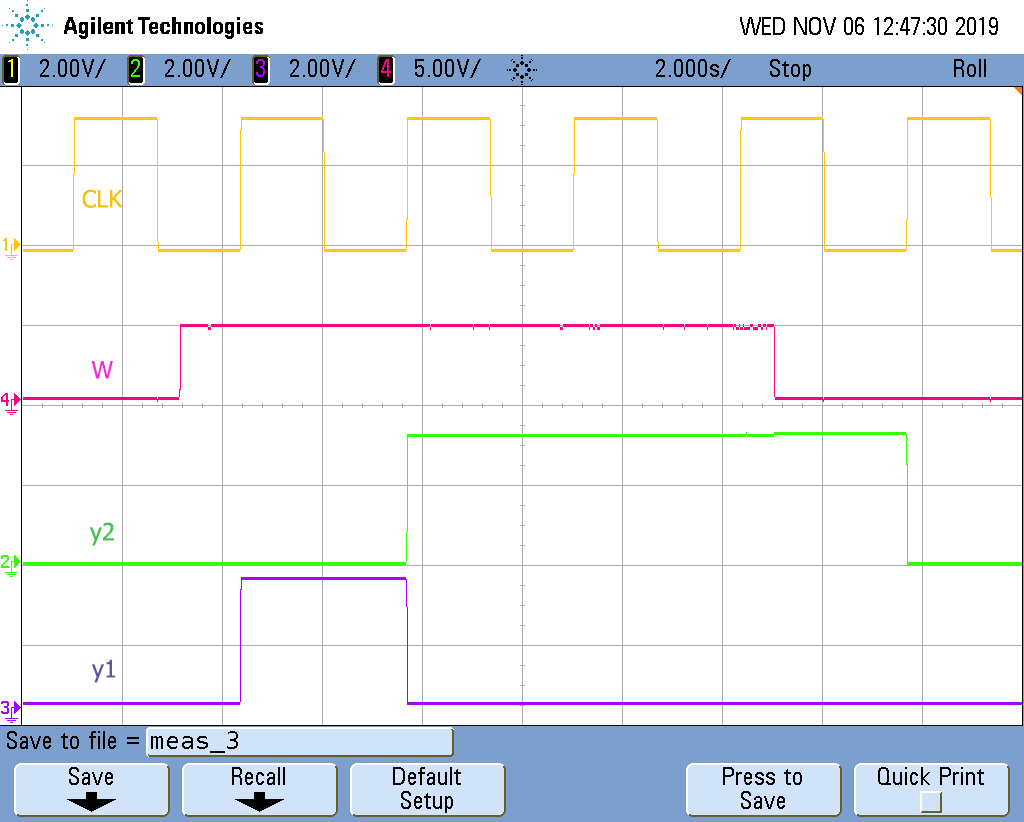
\includegraphics[width=\textwidth,trim={0 3.35cm 0.1cm 1.75cm},clip]{ImagenesEjercicio3/states.png}
\caption{Medición de transiciones de estados: ..00-01-10-...-10-00-..}
\label{states1}
\end{subfigure}
\begin{subfigure}{0.49\textwidth}
\centering
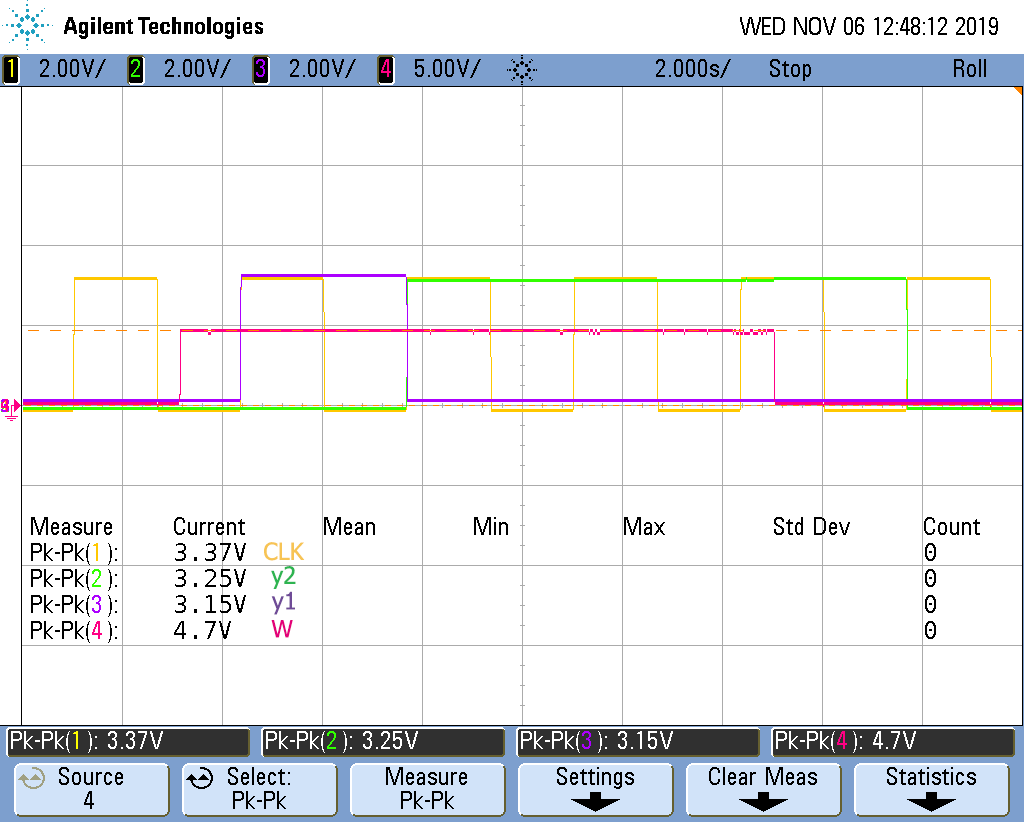
\includegraphics[width=\textwidth,trim={0 3.35cm 0.1cm 1.75cm},clip]{ImagenesEjercicio3/vlevels_states.png}
\caption{Medición de los niveles de tensión.}
\end{subfigure}
\caption{Mediciones del circuito implementado.}
\end{figure}

\begin{figure}[H]
\centering
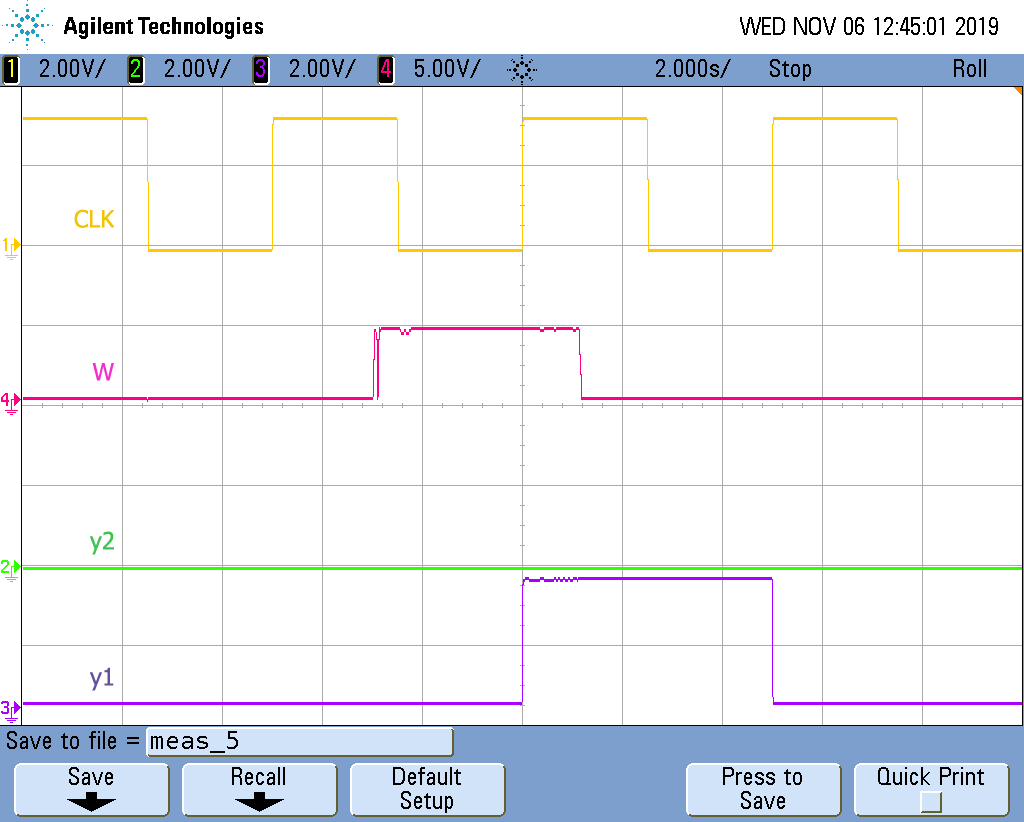
\includegraphics[width=0.7\textwidth,trim={0 3.35cm 0.1cm 1.75cm},clip]{ImagenesEjercicio3/states2.png}
\caption{Medición de la transición de estados: ..00-01-00-..}
\label{states2}
\end{figure}

\begin{figure}[H]
\begin{subfigure}{0.49\textwidth}
\centering
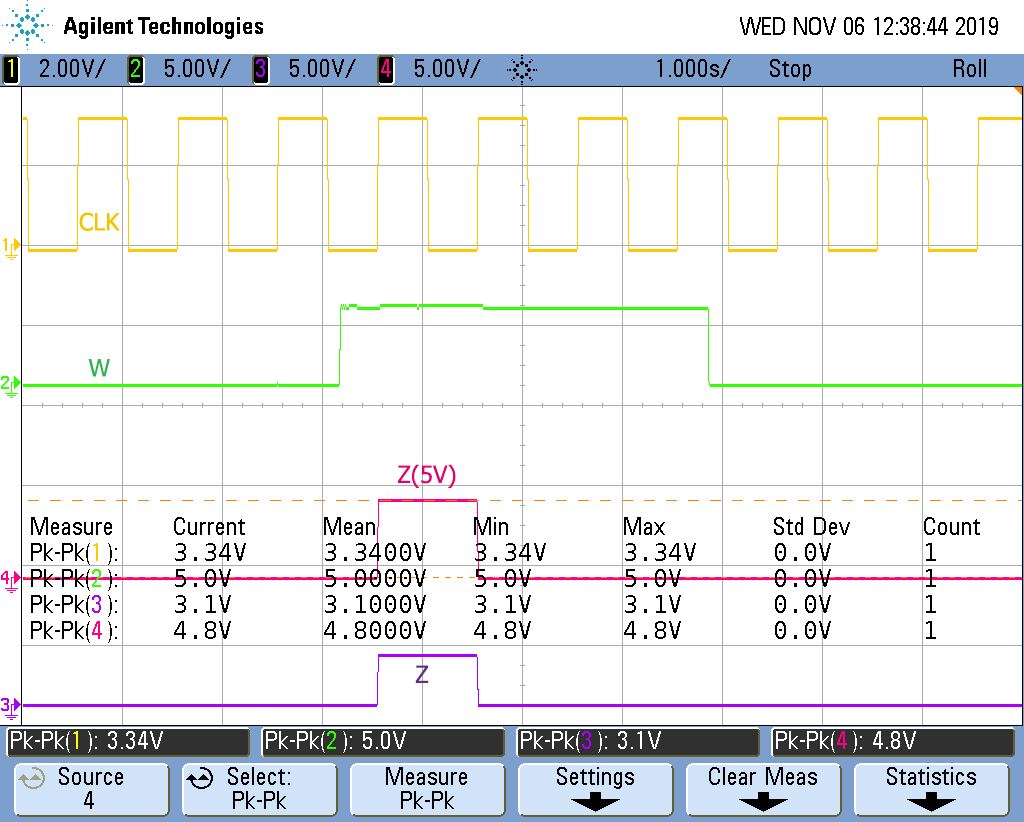
\includegraphics[width=\textwidth,trim={0 3.35cm 0.1cm 1.75cm},clip]{ImagenesEjercicio3/output.png}
\caption{Medición de la transición de la salida del circuito.}
\label{output}
\end{subfigure}
\begin{subfigure}{0.49\textwidth}
\centering
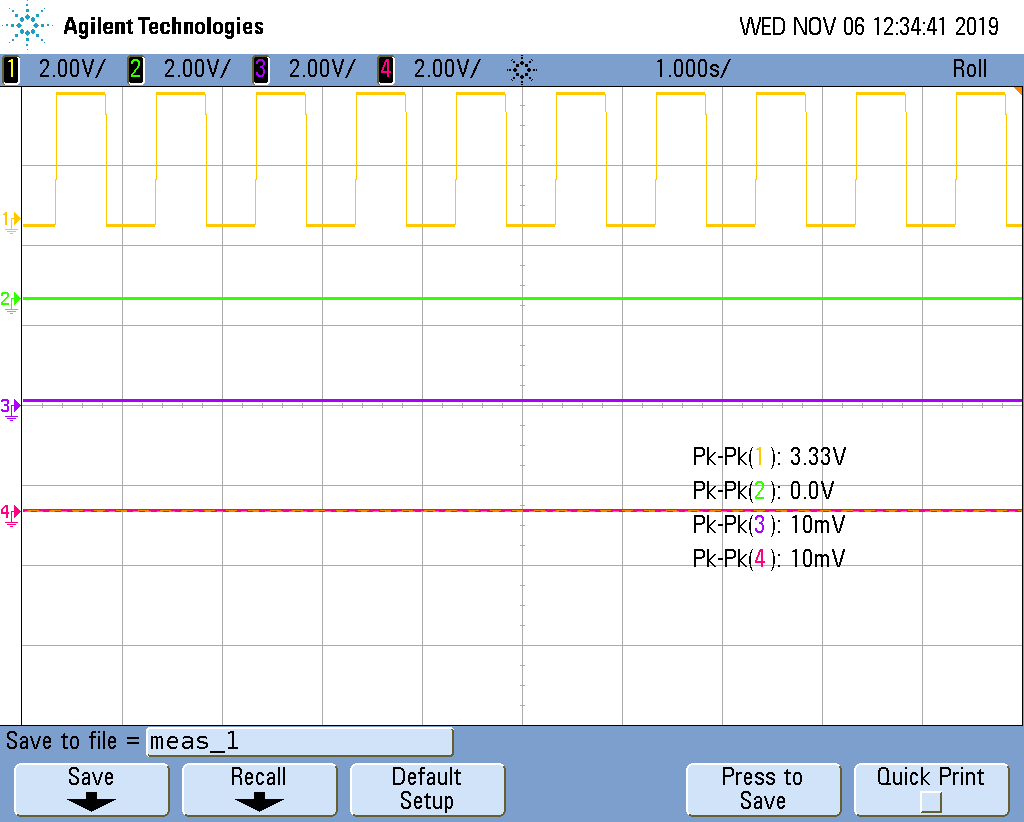
\includegraphics[width=\textwidth,trim={0 3.35cm 0.1cm 1.75cm},clip]{ImagenesEjercicio3/vlevels_low.png}
\caption{Medición de los niveles de tensión en estado bajo..}
\end{subfigure}
\caption{Mediciones del circuito implementado.}
\end{figure}

Se puede observar que el level shifting de niveles de tensión funcionan correctamente. Los niveles de tensión son:
\begin{itemize}
\item $V_{OL} = 10mV$
\item $V_{OH} = 4.8V$
\item $V_{3V3_{H}} = \geq 3.1V$
\item $V_{3V3_{L}} = \approx 0$
\end{itemize}
siendo $V_{3V3}$ el nivel de tensión de la lógica interna del circuito y $V_{OL}$ y $V_{OH}$ los niveles de tensión altos y bajos conseguidos a la salida $Z$.

Luego, se observa en las Figuras (\ref{states1}) y (\ref{states2}) que la transición de estados funciona correctamente habiendo probado todas las combinaciones posibles, y en la Figura (\ref{output}) se observa que la salida posee los valores correctos, siendo cero para todos los estados excepto en el estado $01$ en el cual la salida es igual a un uno lógico. 
El consumo de corriente del circuito es de $15mA$ en todos los estados excepto en el estado $01$ con un consumo de $32mA$.

\subsection{Conclusiones}

Se implementó la FSM propuesta habiendo cumplido los requisitos de niveles de tensión de lógica interna. Si bien la transición de $5V$ a $3V3$ funcionó correctamente, el consumo de corriente es muy elevado siendo este como máximo $32mA$. Si se hubiera querido un consumo menor, se debebería de haber utilizado step-down level-shifters utilizando transistores como se realizó para el step-up level-shifter. Este logró mantener la salida en una tensión muy baja para el estado lógico bajo y en una tensión aceptable para el estado de tensión lógico alto, con un error de $200mV$ por debajo del deseado. Sin embargo, estos niveles de tensión se encuentran totalmente dentro de estándares de márgenes de ruido tanto para la tecnología TTL como para CMOS. Luego, la tensión alta de la lógica interna de $3.1V$ se encuentra también dentro de los márgenes de ruido para ambas tecnologías.


Otras posibles implementaciones para el step-down hubieran sido el uso de un divisor resistivo, lo cual hubiera disminuido mucho el consumo de corriente ya que los valores de resistencias utilizadas posibles hubieran sido cómodamente de unos $10k\Omega$ o más, ya que estos valores no eran lo suficiente altos ni como para generar un divisor resistivo con la impedancia de entrada de la compuerta CMOS ni para generar una corriente comparable con el consumo de estas compuertas. Otra implementación hubiera sido el uso de un comparador ya que este era más barato que un transistor, pero se descartó por su gran tamaño y por poseer implementaciones más simples con mismo resultado.

Finalmente, se concluye que un posible uso de esta maquina de estados implementada es la de obtener un solo pulso a la salida dado el accionar de un botón, teniendo que dejar de oprimir este botón y volver a apretarlo para poder obtener siempre un solo pulso de longitud de un pulso de clock a la salida. Varias modificaciones pueden ser realizadas a esta máquina de estados para obtener otros posibles usos. Por ejemplo, si se deseara implementar la técnica de debouncing para evitar rebotes mecánicos al momento de accionar una entrada se podría redirigir la salida de $w=0$ en el estado $01$ para que esta continúe hacia el próximo estado también y que este último estado mantenga la salida como $z=1$. Así efectivamente por un pulso de clock se ignoran posibles rebotes mecánicos que puedan llegar a poner a la entrada en un estado bajo indeseado. Si un pulso de clock fuese muy poco tiempo debido a su frecuencia se podría repetir el estado $01$ hasta obtener el margen de tiempo deseado.
 

\end{document}


\end{document}